% -*- coding:utf-8 -*-
% vi:encoding=utf-8:
% !TEX encoding = UTF-8 Unicode
%
% This file should be utf8 encoded so that these characters render as
% umlauts: ÄÖÜäöüß
%
%
% FBR_Bericht_2025.tex
%
% Fachbeiratsbericht 2025
% 
% PHENO SECTION

\documentclass{FBR_Bericht_2025}

\setcounter{secnumdepth}{5}
\setcounter{tocdepth}{3}

%\renewcommand{\thechapter}{\Roman{chapter}}
%\renewcommand{\thesection}{\arabic{section}}

\usepackage{physics}

\usepackage[backend=biber,sorting=none]{biblatex}

\addbibresource{Pheno.bib}
%%%%%%%%%%%%%%%%%%%%%%%%%
% PhD_thesis inc file 3
% DEFINITIONS (MiNNLO e acronimi simili)
%%%%%%%%%%%%%%%%%%%%%%%%%

\providecommand{\href}[2]{#2}

\newcommand{\incl}{{\tt inclusive}}
\newcommand{\fidYR}{{\tt fiducial-YR}}
\newcommand{\fidATLAS}{{\tt fiducial-ATLAS}}

\newcommand{\stepone}{{Step\,I}}
\newcommand{\steptwo}{{Step\,II}}
\newcommand{\stepthree}{{Step\,III}}

\newcommand\tS{\tilde{S}}
\newcommand\F{${\textrm F}$}
\newcommand\FJ{${\textrm FJ}$}
\newcommand\FJJ{${\textrm FJJ}$}
\newcommand\PhiBorn{\Phi_{\scriptscriptstyle \textrm B}}
\newcommand\PhiReal{\Phi_{\scriptscriptstyle \textrm R}}
%\newcommand\PhiB{\Phi_{\scriptscriptstyle \textrm H}}
\newcommand\PhiB{\Phi_{\scriptscriptstyle \textrm F}}
\newcommand\PhiBres{\Phi_{\scriptscriptstyle \textrm F,res}}

\newcommand{\flav}{\ell}
\newcommand{\flavBorn}{\flav_{\scriptscriptstyle \textrm B}}
\newcommand{\fullflavBorn}{\hat \flav_{\scriptscriptstyle \textrm B}}
\newcommand{\flavprimeBorn}{\flav'_{\scriptscriptstyle \textrm B}}
\newcommand{\fullflavprimeBorn}{\hat \flav'_{\scriptscriptstyle \textrm B}}
\newcommand{\flavB}{\flav_{\scriptscriptstyle \textrm F}}
\newcommand{\fullflavB}{\hat \flav_{\scriptscriptstyle \textrm F}}
\newcommand{\flavBJ}{\flav_{\scriptscriptstyle \textrm FJ}}
\newcommand{\fullflavBJ}{\hat \flav_{\scriptscriptstyle \textrm FJ}}
\newcommand{\flavBJJ}{\flav_{\scriptscriptstyle \textrm FJJ}}
\newcommand{\fullflavBJJ}{\hat \flav_{\scriptscriptstyle \textrm FJJ}}
\newcommand{\projflav}{\flavB\leftarrow\flavBJ}
\newcommand{\CF}{C_{\mathrm{F}}}
\newcommand{\CA}{C_{\mathrm{A}}}
\newcommand{\NC}{N_{\mathrm{c}}}
\newcommand{\nf}{N_f}
\newcommand{\TF}{T_{\mathrm{F}}}

\newcommand{\flavZg}{\flav_{\scriptscriptstyle Z\gamma}}
\newcommand{\fullflavZg}{\hat \flav_{\scriptscriptstyle Z\gamma}}
\newcommand{\flavZgJ}{\flav_{\scriptscriptstyle Z\gamma {\textrm J}}}
\newcommand{\fullflavZgJ}{\hat \flav_{\scriptscriptstyle Z\gamma {\textrm J}}}
\newcommand{\flavZgJJ}{\flav_{\scriptscriptstyle Z\gamma {\textrm J}}}
\newcommand{\fullflavZgJJ}{\hat \flav_{\scriptscriptstyle Z\gamma {\textrm J}}}
\newcommand{\projflavZg}{\flavZg\leftarrow\flavZgJ}

%\newcommand\PhiBJ{\Phi_{\scriptscriptstyle \textrm HJ}}
\newcommand\PhiBJ{\Phi_{\scriptscriptstyle \textrm FJ}}
\newcommand\ZJ{Z\gamma J}
\newcommand\PhiZJ{\Phi_{\scriptscriptstyle \textrm Z\gamma J}}
\newcommand\PhiBJbar{{\bar \Phi}'_{\scriptscriptstyle \textrm FJ}}
\newcommand\PhiBJJ{\Phi_{\scriptscriptstyle \textrm FJJ}}
\newcommand\PhiZJJ{\Phi_{\scriptscriptstyle \textrm Z\gamma JJ}}
\newcommand\PhiZgam{\Phi_{\scriptscriptstyle \textrm Z\gamma}}
\newcommand{\Fcorr}{F^{\tmop{corr}}_\ell}
\newcommand{\aew}{\alpha_{\text{\scalefont{0.77}EW}}} 
\newcommand{\aw}{\alpha_w}
\newcommand{\asCMW}{\alpha_s^{\textrm †CMW}}
%\newcommand{\cO}[1]{{\cal O}\left(#1\right)}
\newcommand{\NNLL}{\text{NNLL}}
\newcommand{\eff}{\epsilon}
\newcommand{\ee}{\ell^+\ell^-}
\newcommand{\kt}[1]{k_{\scaleto{\textrm T}{4pt},#1}}
\newcommand{\veckt}[1]{\vec{k}_{\scaleto{\textrm T}{4pt},#1}}
%\newcommand{\dk}[1]{\langle \mathd k_{#1}\rangle}
\newcommand{\fullF}{\mathcal{F}}
\newcommand{\FNLL}{\mathcal{F}_{\textrm NLL}}
\newcommand{\FNNLL}{\mathcal{F}_{\textrm NNLL}}
\newcommand{\css}{\text{\scriptsize CSS}}
\newcommand{\zi}{z_i^{(\ell_i)}}
\newcommand{\pt}{p_{\text{\relscale{0.77}T}}}
\newcommand{\GZ}{{\Gamma_Z}}
\newcommand{\GW}{{\Gamma_W}}
\newcommand{\thW}{{\theta_W}}
\newcommand{\mtop}{{m_{\text{\relscale{0.77}top}}}}
\newcommand{\qt}{{q_{\text{\relscale{0.77}T}}}}
\newcommand{\ptarg}[1]{{p_{\text{\relscale{0.77}T,$#1$}}}}
\newcommand{\marg}[1]{{m_{\text{\relscale{0.77}$#1$}}}}
\newcommand{\ptg}{p_{\text{\relscale{0.77}T,$\gamma$}}}
\newcommand{\ptgcut}{{p_{\text{\relscale{0.77}T,$\gamma$}}^{\textrm cut}}}
\newcommand{\ptjcut}{{p_{\text{\relscale{0.77}T,$j$}}^{\textrm cut}}}

%%newdef
\newcommand{\ptjmin}{\bar{p}_{\text{\relscale{0.77}T,$j$}}}
\newcommand{\ptgmin}{\bar{p}_{\text{\relscale{0.77}T,$\gamma$}}}
\newcommand{\ptgone}{p_{\text{\relscale{0.77}T,$\gamma_1$}}}
\newcommand{\ptgtwo}{p_{\text{\relscale{0.77}T,$\gamma_2$}}}
\newcommand{\ptgthree}{p_{\text{\relscale{0.77}T,$\gamma_3$}}}

\newcommand{\ptr}{{p_{\text{\relscale{0.77}T}}}^{\text{\relscale{0.9}r}}}
\newcommand{\ptrad}{{p_{\text{\relscale{0.77}T,rad}}}}
\newcommand{\pth}{{p_{\text{\relscale{0.77}T,$H$}}}}
\newcommand{\ptz}{{p_{\text{\relscale{0.77}T,$Z$}}}}
\newcommand{\ptw}{{p_{\text{\relscale{0.77}T,$W$}}}}
\newcommand{\ptnu}{{p_{\text{\relscale{0.77}T,$\nu$}}}}
\newcommand{\mtwz}{{m_{\text{\relscale{0.77}T,$WZ$}}}}
\newcommand{\dphiwz}{{\Delta\phi_{\text{\relscale{0.77}$WZ$}}}}
\newcommand{\dyZlW}{{|y_{\text{\relscale{0.77}$Z$}}-y_{\text{\relscale{0.77}$
\ell_W$}}|}}
\newcommand{\ptww}{{p_{\text{\relscale{0.77}T,$WW$}}}}
\newcommand{\ptwp}{{p_{\text{\relscale{0.77}T,$W^+$}}}}
\newcommand{\ptwm}{{p_{\text{\relscale{0.77}T,$W^-$}}}}
\newcommand{\mtww}{{m_{\text{\relscale{0.77}T,$WW$}}}}
\newcommand{\mtwwexp}{{m_{\text{\relscale{0.77}T,$WW$}}^{\textrm exp}}}
\newcommand{\ptllg}{{p_{\text{\relscale{0.77}T,}\ell\ell\gamma}}}
\newcommand{\ptzg}{\ptllg}
\newcommand{\ptll}{{p_{\text{\relscale{0.77}T,$e^+e^-$}}}}
\newcommand{\ptlnu}{{p_{\text{\relscale{0.77}T,$\mu\nu_\mu$}}}}
\newcommand{\ptj}{p_{\text{\relscale{0.77}T,$j$}}}
\newcommand{\ptjone}{{p_{\text{\relscale{0.77}T,$j_1$}}}}
\newcommand{\ptjoneveto}{{p_{\text{\relscale{0.77}T,$j_1$}}^{\textrm veto}}}
\newcommand{\ptjtwo}{{p_{\text{\relscale{0.77}T,$j_2$}}}}
\newcommand{\ptlm}{{p_{\text{\relscale{0.77}T,$\ell^-$}}}}
\newcommand{\ptl}{{p_{\text{\relscale{0.77}T,$\ell$}}}}
\newcommand{\ptlone}{{p_{\text{\relscale{0.77}T,$\ell_1$}}}}
\newcommand{\ptltwo}{{p_{\text{\relscale{0.77}T,$\ell_2$}}}}
\newcommand{\ptmiss}{{p_{\text{\relscale{0.77}T,miss}}}}
\newcommand{\ptmissrel}{{p_{\text{\relscale{0.77}T,miss,rel}}}}
\newcommand{\yh}{{y_{\text{\relscale{0.77}H}}}}
\newcommand{\yz}{{y_{\text{\relscale{0.77}Z}}}}
\newcommand{\ywp}{{y_{\text{\relscale{0.77}$W^+$}}}}
\newcommand{\yl}{{y_{\text{\relscale{0.77}$\ell$}}}}
\newcommand{\ylone}{{y_{\text{\relscale{0.77}$\ell_1$}}}}
\newcommand{\dphill}{{\Delta\phi_{\text{\relscale{0.77}$\ell_1\ell_2$}}}}
\newcommand{\yww}{{y_{\text{\relscale{0.77}$WW$}}}}
\newcommand{\yjone}{{y_{\text{\relscale{0.77}$j_1$}}}}
\newcommand{\dyww}{{\Delta y_{\text{\relscale{0.77}$W^-,W^+$}}}}
\newcommand{\mh}{{m_{\text{\relscale{0.77}H}}}}
\newcommand{\mz}{{m_{\text{\relscale{0.77}Z}}}}
\newcommand{\mw}{{m_{\text{\relscale{0.77}W}}}}
\newcommand{\mww}{{m_{\text{\relscale{0.77}WW}}}}
\newcommand{\mwsq}{{m^2_{\text{\relscale{0.77}W}}}}
\newcommand{\mt}{{m_{\text{\relscale{0.77}t}}}}
\newcommand{\mT}{{m_{\text{\relscale{0.77}T}}}}
\newcommand{\mgj}{{m_{\text{\relscale{0.77}$\gamma j_1$}}}}
\newcommand{\mllg}{{m_{\text{\relscale{0.77}$\ell\ell\gamma$}}}}
\newcommand{\mlnu}{{m_{\text{\relscale{0.77}$\mu\nu_\mu$}}}}
\newcommand{\etal}{{\eta_{\text{\relscale{0.77}$\ell$}}}}
\newcommand{\etallg}{{\eta_{\text{\relscale{0.77}$\ell\ell\gamma$}}}}
\newcommand{\etalone}{{\eta_{\text{\relscale{0.77}$\ell_1$}}}}
\newcommand{\etaltwo}{{\eta_{\text{\relscale{0.77}$\ell_2$}}}}
\newcommand{\etag}{{\eta_{\text{\relscale{0.77}$\gamma$}}}}
\newcommand{\etaj}{{\eta_{\text{\relscale{0.77}j}}}}
\newcommand{\etah}{{\eta_{\text{\relscale{0.77}H}}}}
\newcommand{\detallgj}{{\Delta\eta_{\text{\relscale{0.77}$\ell\ell\gamma, j_1$}}}}
\newcommand{\dphillg}{{\Delta\phi_{\text{\relscale{0.77}$\ell\ell,\gamma$}}}}
\newcommand{\drlg}{{\Delta R_{\text{\relscale{0.77}$\ell \gamma$}}}}
\newcommand{\drgjone}{{\Delta R_{\text{\relscale{0.77}$\gamma j_1$}}}}
\newcommand{\drgjtwo}{{\Delta R_{\text{\relscale{0.77}$\gamma j_2$}}}}
\newcommand{\drej}{{\Delta R_{\text{\relscale{0.77}$e j$}}}}

%new def
\newcommand{\rjg}{R_{\text{\relscale{0.77}$j \gamma$}}}
\newcommand{\rjgone}{R_{\text{\relscale{0.77}$j \gamma_1$}}}
\newcommand{\rjgtwo}{R_{\text{\relscale{0.77}$j \gamma_2$}}}
\newcommand{\rjgthree}{R_{\text{\relscale{0.77}$j \gamma_3$}}}
\newcommand{\rjgmin}{\bar{R}_{\text{\relscale{0.77}$j \gamma$}}}
\newcommand{\rjonegone}{R_{\text{\relscale{0.77}$j_1 \gamma_1$}}}
\newcommand{\rjonegtwo}{R_{\text{\relscale{0.77}$j_1 \gamma_2$}}}
\newcommand{\rjonegthree}{R_{\text{\relscale{0.77}$j_1 \gamma_3$}}}
\newcommand{\rjtwogone}{R_{\text{\relscale{0.77}$j_2 \gamma_1$}}}
\newcommand{\rjtwogtwo}{R_{\text{\relscale{0.77}$j_2 \gamma_2$}}}
\newcommand{\rjtwogthree}{R_{\text{\relscale{0.77}$j_2 \gamma_3$}}}


\newcommand{\lw}{\ensuremath{\mu}}
\newcommand{\lpw}{\ensuremath{\ell^+_{\text{\relscale{0.77}W}}}}
\newcommand{\lmw}{\ensuremath{\ell^-_{\text{\relscale{0.77}W}}}}
\newcommand{\lpmw}{\ensuremath{\ell^{\pm}_{\text{\relscale{0.77}W}}}}

\newcommand{\lz}{\ensuremath{e}}
\newcommand{\lpz}{\ensuremath{e^+}}
\newcommand{\lmz}{\ensuremath{e^-}}
\newcommand{\lpmz}{\ensuremath{e^{\pm}_{\text{\relscale{0.77}}}}}
\newcommand{\lzlead}{\ensuremath{e_{\text{\relscale{0.77}Z,1}}}}
\newcommand{\lzsubl}{\ensuremath{e_{\text{\relscale{0.77}Z,2}}}}

\newcommand{\ptlz}{\ensuremath{p_{\text{\relscale{0.77}T,\lz}}}}
\newcommand{\ptlw}{\ensuremath{p_{\text{\relscale{0.77}T,\lw}}}}
\newcommand{\ptlzlead}{\ensuremath{p_{\text{\relscale{0.77}T,\lzlead}}}}
\newcommand{\ptlzsubl}{\ensuremath{p_{\text{\relscale{0.77}T,\lzsubl}}}}

\newcommand{\mlll}{\ensuremath{m_{\text{\relscale{0.77}$3\ell$}}}}
\newcommand{\mwz}{\ensuremath{m_{\text{\relscale{0.77}WZ}}}}
\newcommand{\mtw}{\ensuremath{m_{\text{\relscale{0.77}T,W}}}}
\newcommand{\ptwz}{\ensuremath{p_{\text{\relscale{0.77}T,WZ}}}}
\newcommand{\ptlp}{\ensuremath{p_{\text{\relscale{0.77}T,\ell'}}}}
\newcommand{\dRll}{\ensuremath{\Delta R_{\text{\relscale{0.77}$\ell\ell$}}}}
\newcommand{\dRllp}{\ensuremath{\Delta R_{\text{\relscale{0.77}$\ell\ell'$}}}}
\newcommand{\etalp}{\ensuremath{\eta_{\text{\relscale{0.77}$\ell'$}}}}

\newcommand{\qcdfull}{\ensuremath{\text{NNLO}_{\textrm QCD}^{{\textrm (QCD,QED)}_{\textrm PS}}}}
\newcommand{\qcdqcd}{\ensuremath{\text{NNLO}_{\textrm QCD}^{{\textrm (QCD)}_{\textrm PS}}}}

\newcommand{\addfull}{\ensuremath{\text{NNLO}_{\textrm QCD}^{\textrm (QCD,QED)_{\textrm PS}} + \delta{\textrm NLO}_{\textrm EW}^{\textrm (QCD,QED)_{\textrm PS}}}}
\newcommand{\addqcdfull}{\ensuremath{\text{NNLO}_{\textrm QCD}^{\textrm (QCD,QED)_{\textrm PS}} + \delta{\textrm NLO}_{\textrm EW}^{\textrm (QED)_{\textrm PS}}}}
\newcommand{\addqedfull}{\ensuremath{\text{NLO}_{\textrm EW}^{\textrm (QCD,QED)_{\textrm PS}} + \delta{\textrm NNLO}_{\textrm QCD}^{\textrm (QCD)_{\textrm PS}}}}

\newcommand{\multfull}{\ensuremath{\text{NNLO}_{\textrm QCD}^{\textrm (QCD,QED)_{\textrm PS}} \times \text{K-NLO}_{\textrm EW}^{\textrm (QCD,QED)_{\textrm PS}}}}
\newcommand{\multqcdfull}{\ensuremath{\text{NNLO}_{\textrm QCD}^{\textrm (QCD,QED)_{\textrm PS}} \times \text{K-NLO}_{\textrm EW}^{\textrm (QED)_{\textrm PS}}}}
\newcommand{\multqedfull}{\ensuremath{\text{NLO}_{\textrm EW}^{\textrm (QCD,QED)_{\textrm PS}} \times \text{K-NNLO}_{\textrm QCD}^{\textrm (QCD)_{\textrm PS}}}}

\newcommand{\multmatrix}{\ensuremath{\text{NNLO}_{\textrm QCD}^{\textrm (QCD)_{\textrm PS}} \times \text{K-NLO}_{\textrm EW}^{\text{\Matrix{}}}}}
\newcommand{\QCDpEW}{\ensuremath{ \text{NNLO}_{\textrm QCD+EW}^{\textrm (QCD, QED)_{\textrm PS}}}} 
\newcommand{\QCDtEW}{\ensuremath{ \text{NNLO}_{\textrm QCDxEW}^{\textrm (QCD, QED)_{\textrm PS}}}} 
\newcommand{\QCDtEWfo}{\ensuremath{ \text{NNLO}_{\textrm QCD}^{\textrm (QCD)_{\textrm PS}} \times \text{K-NLO}_{\textrm EW}^{\textrm (f.o.)}}} 



\newcommand{\drlj}{{\Delta R_{\text{\relscale{0.77}$\ell,j$}}}}
\newcommand{\drgj}{{\Delta R_{\text{\relscale{0.77}$\gamma j$}}}}
\newcommand{\drgjo}{{\Delta R_{\text{\relscale{0.77}$\gamma j_1$}}}}
\newcommand{\drgjt}{{\Delta R_{\text{\relscale{0.77}$\gamma j_2$}}}}
\newcommand{\fcl}{{E_{\text{\relscale{0.77}T}}^{\text{\relscale{0.77}cone$0.2$}}/p_{\text{\relscale{0.77}T},\gamma}}}
\newcommand{\muF}{{\mu_{\text{\relscale{0.77}F}}}}
\newcommand{\muR}{{\mu_{\text{\relscale{0.77}R}}}}
\newcommand{\muFtwo}{{\mu^2_{\text{\relscale{0.77}F}}}}
\newcommand{\muRtwo}{{\mu^2_{\text{\relscale{0.77}R}}}}
\newcommand{\muFc}{{\mu_{\text{\relscale{0.77}F},0}}}
\newcommand{\muRc}{{\mu_{\text{\relscale{0.77}R},0}}}
\newcommand{\muRy}{{\mu_{\text{\relscale{0.77}R}}^{(0),y}}}
\newcommand{\muRb}{{\mu_{\text{\relscale{0.77}R}}^{(0),\alpha}}}
\newcommand{\KF}{K_{\text{\relscale{0.77}F}}}
\newcommand{\KR}{K_{\text{\relscale{0.77}R}}}
\newcommand{\KRy}{{K^y_{\text{\relscale{0.77}R}}}}
\newcommand{\KQ}{{K_{\text{\relscale{0.77}Q}}}}
\newcommand{\Q}{{Q_{\text{\relscale{0.77}$0$}}}}
\newcommand{\Qc}{{Q_{\text{\relscale{0.77}res},0}}}

\newcommand{\noun}[1]{{\scshape #1}}
\newcommand{\MADGRAPH}{\noun{MadGraph v4}}
\newcommand{\GOSAM}{\noun{GoSam 2.0}}
\newcommand{\POWHEG}{\noun{Powheg}}
\newcommand{\POWHEGMiNLO}{\noun{Powheg-MiNLO}}
\newcommand{\POWHEGBOX}{\noun{Powheg-Box}}
\newcommand{\POWHEGBOXRES}{\noun{Powheg-Box-Res}}
\newcommand{\POWHEGBOXVTWO}{\noun{Powheg-Box-V2}}
\newcommand{\minlobare}{{\noun{MiNLO}}}
\newcommand{\minlosimple}{{\noun{MiNLO}}}
\newcommand{\minlo}{{\noun{MiNLO$^{\prime}$}}}
\newcommand{\minnlo}{{\noun{MiNNLO$_{\textrm{PS}}$}}}
\newcommand{\Matrix}{{\noun{Matrix}}}
\newcommand{\OpenLoops}{{\noun{OpenLoops}}}
\newcommand{\PYTHIA}[1]{\noun{Pythia{#1}}}

\newcommand{\NNLOps}{NNLO+PS}
\newcommand{\fnnlo}{NNLO}
\newcommand{\NLOps}{NLO+PS}
\newcommand{\setupinclusive}{{\tt inclusive setup}}
\newcommand{\setupfiducial}{{\tt fiducial setup}}
\newcommand{\setupatlas}{{\tt ATLAS setup}}

\newcommand{\abar}{\frac{\as}{2\pi}}
\newcommand{\abarmu}[1]{\frac{\as(#1)}{2\pi}}

\newcommand{\Vsc}{V}
\newcommand{\Vwa}{V_{\textrm wa}}
\newcommand{\Vfull}{V}
\newcommand{\wzc}{V_{\textrm hc}}
\newcommand{\Vr}{V_{r}}
\newcommand{\ptB}{p_{t}^{(B)}}

\newcommand{\dZ}{d{\cal Z}[\{R', k_i\}]}
\newcommand{\RpNLL}{R'_{\mathrm{NLL}}}

\newcommand{\LambdaPWG}{\Lambda_{\textrm pwg}}

\newcommand{\yll}{{y_{\text{\relscale{0.77}\ell\ell}}}}
\newcommand{\mll}{{m_{\text{\relscale{0.77}\ell\ell}}}}
\newcommand{\mQQF}{m_{Q\bar Q{\textrm F}}}
\newcommand{\muQ}{\mu_{Q}}
\newcommand{\Mdiv}{\mathcal{M}^\textrm{IR-div}}
\newcommand{\phs}{\ensuremath{\phi^{*}_\eta}\xspace}



\usepackage{xcolor}
\newcommand{\mathd}{\mathrm{d}}
\newcommand{\tmop}[1]{\ensuremath{\operatorname{#1}}}
\newenvironment{enumeratealpha}{\begin{enumerate}[a{\textup{)}}] }{\end{enumerate}}
\newenvironment{itemizedot}{\begin{itemize} \renewcommand{\labelitemi}{$\bullet$}\renewcommand{\labelitemii}{$\bullet$}\renewcommand{\labelitemiii}{$\bullet$}\renewcommand{\labelitemiv}{$\bullet$}}{\end{itemize}}
\newcommand{\Eta}{\mathrm{H}}
\newcommand{\tmverbatim}[1]{{\ttfamily{#1}}}

\def\collr{orange}
\def\colsp{blue}
\def\colmw{purple}
\def\colsk{cyan}
\def\coldr{red}
\def\colpt{red}
\def\colgz{red}
\def\coljl{magenta}
\def\colsz{violet}
\def\colcb{brown}
\def\colas{magenta}
\def\coljm{cyan}


\newcommand{\mwcom}[1]{\textit{\textcolor{\colmw}{\{MW: #1 \}}}}
\newcommand{\gzcom}[1]{\textit{\textcolor{\colpt}{\{GZ: #1 \}}}}
\newcommand{\cbcom}[1]{\textit{\textcolor{\colcb}{\{CB: #1 \}}}}
\newcommand{\ascom}[1]{\textit{\textcolor{\colas}{\{AS: #1 \}}}}
\newcommand{\jmcom}[1]{\textit{\textcolor{\coljm}{\{JM: #1 \}}}}

\newcommand{\asdel}[1]{\textcolor{\colas}{\sout{#1}}}
\newcommand{\mwdel}[1]{\textcolor{\colmw}{\sout{#1}}}
\newcommand{\gzdel}[1]{\textcolor{\colmg}{\sout{#1}}}
\newcommand{\jmdel}[1]{\textcolor{\coljm}{\sout{#1}}}

\newcommand{\mwadd}[2]{\textcolor{\colmw}{\sout{#1}#2}}
\newcommand{\asadd}[2]{\textcolor{\colas}{\sout{#1}#2}}
\newcommand{\cbadd}[2]{\textcolor{\colcb}{\sout{#1}#2}}
\newcommand{\gzadd}[2]{\textcolor{\colgz}{\sout{#1}#2}}
\newcommand{\jmadd}[2]{\textcolor{\coljm}{\sout{#1}#2}}


\def\ltap{\raisebox{-.6ex}{\rlap{$\,\sim\,$}} \raisebox{.4ex}{$\,<\,$}} 
\def\gtap{\raisebox{-.6ex}{\rlap{$\,\sim\,$}} \raisebox{.4ex}{$\,>\,$}} 
\def\lra{\leftrightarrow} 
\def\naive{na\"{\i}ve} 
%\newcommand\as{\alpha_{\mathrm{S}}} 
%\newcommand\f[2]{\frac{#1}{#2}} 
\def\bom#1{{\mbox{\boldmath $#1$}}} 
\def\to{\rightarrow}
\def\ito{\leftarrow} 
\def\nn{\nonumber} 
\def\mbbggs{m_{2b2\gamma}^{\star}}
\def\arrowlimit#1{\mathrel{\mathop{\longrightarrow}\limits_{#1}}} 
\def\ptmin{p_{T}^{\textrm min}}
\def\ptmax{p_{T}^{\textrm max}}
\def\ptveto{p_{T,\ell\ell\gamma}^{\textrm veto}}
\def\ep{\epsilon}
\def\ms{${\overline {\textrm MS}}$}
\def\perc{\%}
\def\mH{m_H}
\def\mb{m_b}
\def\mt{m_t}
\def\mw{m_W}
\def\mz{m_Z}
\def\qT{q_T}
%\def\pT{p_T}
\def\GeV{\mathrm{GeV}}
\def\TeV{\mathrm{TeV}}
\def\tL{{\widetilde L}}

\newcommand{\eqn}[1]{eq.\,(\ref{#1})}
\newcommand{\neqn}[1]{eqs.\,(\ref{#1})}
\newcommand{\fig}[1]{figure\,\ref{#1}}
\newcommand{\figs}[1]{figures\,\ref{#1}}
\newcommand{\tab}[1]{table\,\ref{#1}}
\newcommand{\sct}[1]{section\,\ref{#1}}
\newcommand{\scts}[1]{sections\,\ref{#1}}
\newcommand{\app}[1]{appendix\,\ref{#1}}

\def\refeq#1{\mbox{eq.\,\eqref{#1}}}
\def\refeqs#1{\mbox{eqs.\,\eqref{#1}}}
\def\reffi#1{\mbox{figure\,\ref{#1}}}
\def\reffitwo#1#2{\mbox{figures\,\ref{#1} and \ref{#2}}}
\def\reffis#1#2{\mbox{figures\,\ref{#1}--\ref{#2}}}
\def\refta#1{\mbox{table\,\ref{#1}}}
\def\reftatwo#1#2{\mbox{tables\,\ref{#1} and \ref{#2}}}
\def\reftas#1{\mbox{tables\,\ref{#1}}}
\def\refse#1{\mbox{section\,\ref{#1}}}
\def\refsetwo#1#2{\mbox{sections\,\ref{#1} and \ref{#2}}}
\def\refses#1{\mbox{sections\,\ref{#1}}}
\def\refapp#1{\mbox{app.\,\ref{#1}}}
\def\citere#1{\mbox{ref.\,\cite{#1}}}
\def\citeres#1{\mbox{refs.\,\cite{#1}}}


\newcommand{\rcut}{\ensuremath{r_{\mathrm{cut}}}}
%\newcommand{\zz}{\ensuremath{ZZ}}
\newcommand{\ww}{\ensuremath{W^+W^-}}
\newcommand{\wz}{\ensuremath{W^\pm Z}}
\newcommand{\wpz}{\ensuremath{W^+Z}}
\newcommand{\wmz}{\ensuremath{W^-Z}}
\newcommand{\z}{\ensuremath{Z}}
\newcommand{\w}{\ensuremath{W}}

\newcommand{\abbrev}{}
\newcommand{\llog}{\text{\abbrev LL}}
\newcommand{\nll}{\text{\abbrev NLL}}
\newcommand{\nnll}{\text{\abbrev NNLL}}
\newcommand{\lo}{\text{\abbrev LO}}
\newcommand{\nlo}{\text{\abbrev NLO}}
\newcommand{\nnlo}{\text{\abbrev NNLO}}
\newcommand{\nlonll}{\nlo\plus\nll}
\newcommand{\nnlonnll}{\nnlo\plus\nnll}
\newcommand{\qcd}{{\abbrev QCD}}
\newcommand{\D}{\mathrm{d}}

\newcommand{\cme}{centre-of-mass energy}
\newcommand{\cmes}{centre-of-mass energies}

\newcommand\Tstrut{\rule{0pt}{3.0ex}}         % = `top' strut
\newcommand\Bstrut{\rule[-1.5ex]{0pt}{0pt}}   % = `bottom' strut

\interfootnotelinepenalty=10000
%\setlength{\parindent}{0pt}

\newcommand\mlbl[1]{{\mbox{\footnotesize #1}}} 

\newcommand{\elle}{\ensuremath{\ell}}
\newcommand{\genllln}{\ensuremath{\elle\elle\elle\nu}}
\newcommand{\llln}{\elle'^\pm{\nu}_{\elle^\prime} \elle^-\elle^+}
\newcommand{\mllln}{\ensuremath{m_{\llln}}}
\newcommand{\ptllln}{\ensuremath{p_{T,\llln}}}


\setlength{\tabcolsep}{5pt}

\usepackage{etoolbox}
\makeatletter
% \tracingpatches
\patchcmd{\@sect}{#8}{\boldmath #8}{}{}
\let\ori@chapter\@chapter
\def\@chapter[#1]#2{\ori@chapter[\boldmath#1]{\boldmath#2}}
\makeatother




\newcommand{\gev}[1]{$\unit{#1}{\giga\electronvolt}$}
\newcommand{\tev}[1]{$\unit{#1}{\tera\electronvolt}$}

\newcommand{\gevm}[1]{\unit{#1}{\giga\electronvolt}}
\newcommand{\tevm}[1]{\unit{#1}{\tera\electronvolt}}

\newcommand{\half}{$\frac{1}{2}$}

\newcommand{\ddk}[1]{\frac{d^d k_{#1}}{(4\pi)^d}}
\newcommand{\sidenote}[1]{\todo[noline]{#1}}

\newcommand\calo[1]{{\cal O}\hspace{-0.2em}\left(#1\right)}

\newcommand{\cala}{{\cal A}}
\newcommand{\bbH}{\ensuremath{b\bar{b}\text{H}}}
\newcommand{\bbtoH}{\ensuremath{b\bar{b}\rightarrow\text{H}}}
\newcommand{\ttH}{\ensuremath{t\bar{t}\text{H}}}
\newcommand{\bbphi}{\ensuremath{b\bar{b}\phi}}
\newcommand{\yt}{\ensuremath{y_t}}
\newcommand{\ytsq}{\ensuremath{y_t^2}}
\newcommand{\yb}{\ensuremath{y_b}}
\newcommand{\ybsq}{\ensuremath{y_b^2}}
\newcommand{\ybyt}{\ensuremath{y_b\, y_t}}


%%% feb15, 2025 - definitions %%%%
\newcommand{\phiF}{\Phi_{\text{F}}}
\newcommand{\phirad}{\Phi_{\text{rad}}}
\newcommand{\phiFJ}{\Phi_{\text{FJ}}}
\newcommand{\obs}{\mathcal{O}}
\newcommand{\barphiF}{\bar{\Phi}_{\text{F}}}
\newcommand{\barphiFJ}{\bar{\Phi}_{\text{FJ}}}
\newcommand{\dpwg}{\Delta_{\text{pwg}}}
\newcommand{\lpwg}{\Lambda_{\text{pwg}}}
\newcommand{\ptF}{{p_{\text{\relscale{0.77}T,$F$}}}}
\newcommand{\phiFJJ}{\Phi_{\text{FJJ}}}
\newcommand{\meF}{M_{\scriptscriptstyle\mathrm F}}
\newcommand{\meFJ}{M_{\scriptscriptstyle\mathrm FJ}}

\newcommand{\phiQQF}{\Phi_{\text{X}}}
\newcommand{\phiQQFJ}{\Phi_{\text{XJ}}}
\newcommand{\phiQQFJJ}{\Phi_{\text{XJJ}}}
\newcommand{\cflavF}{c_{\text{X}}}
\newcommand{\cflavFJ}{c_{\text{XJ}}}
\newcommand{\cflavFJJ}{c_{\text{XJJ}}}

\newcommand{\msb}{\overline{\text{MS}}}

\newcommand{\muIR}{{\mu_{\text{\relscale{0.77}S}}}}
\newcommand{\muRuno}{{\mu_{\text{\relscale{0.77}R,1}}}}
\newcommand{\muRdue}{{\mu_{\text{\relscale{0.77}R,2}}}}
\newcommand{\muIRuno}{{\mu_{\text{\relscale{0.77}S,1}}}}
\newcommand{\muIRdue}{{\mu_{\text{\relscale{0.77}S,2}}}}
\newcommand{\muRunotwo}{{\mu^2_{\text{\relscale{0.77}R,1}}}}
\newcommand{\muRduetwo}{{\mu^2_{\text{\relscale{0.77}R,2}}}}
\newcommand{\muIRunotwo}{{\mu^2_{\text{\relscale{0.77}S,1}}}}
\newcommand{\muIRduetwo}{{\mu^2_{\text{\relscale{0.77}S,2}}}}


\begin{document}

\onecolumn
\pdfbookmark[1]{Table of Contents}{table_of_contents}
\tableofcontents
\cleardoublepage

\twocolumn

% ----------------------------------------------------------------------
\chapter{Research Activities -- Theory}
% ----------------------------------------------------------------------
\section[Novel computational techniques in particle physics and phenomenological applications]{Novel computational techniques in particle physics and phenomenological applications}
% ----------------------------------------------------------------------
\begin{Namen}
Director: Prof. Dr. G. Zanderighi
\end{Namen}

The research focus of this group is towards pushing the precision of
theoretical predictions for colliders processes and providing
practical predictions and tools to be used for comparisons of data and
theory.

Currently, the group consists of two group leaders, one senior
postdoc, six postdocs (one funded by the TUM), as well as
four PhD students. Some of these researchers joined the group during this
reporting period, while others have left since the last reporting
period. This report covers the activity of all group members (old and new) while at MPP. 


%%%%%%%%%%%%%%%%%%%%%%%%%%%%%%%%%%%%%%%%%%%%%%%%%%%%%%%%%%%%%%%%%%%%%%
\subsection{Novel event simulations for hadron--hadron collisions}
%%%%%%%%%%%%%%%%%%%%%%%%%%%%%%%%%%%%%%%%%%%%%%%%%%%%%%%%%%%%%%%%%%%%%%
\begin{refsection}
Full fledged simulations of hadron-level events build the theoretical 
core of any experimental analyses performed at colliders.
By closing the gap between the measured data in the experimental
detectors and the theoretical predictions based on quantum-field theory
(QFT) computations, event generators are one of central tools developed
in particle theory. In addition, their predictions provide a realistic description
of any infrared-safe observable in comparison to data.

To keep up with the steadily decreasing experimental uncertainties, it is 
mandatory to develop event simulations at the highest possible accuracy.
This can be achieved by improving the perturbative all-order description 
of parton showers, on the one hand, and by including higher-order corrections
in the event simulations on the other. This will allows us ultimately to observe even the smallest
deviations from SM predictions and paves a way towards observing new-physics phenomena.

Event generators with next-to-leading order (NLO) QCD accuracy have been the standard for several years. 
However, there has been a substantial progress in achieving next-to-NLO
(NNLO) event simulations in the past years, much of which has been driven by our research
group. The \minnlo{} method to match NNLO predictions with parton showers (NNLO+PS)
was introduced by us in 2019 for $2\to 1$ colour-singlet 
processes \cite{Monni:2019whf,Monni:2020nks}, generalized $2\to 2$ reactions 
(and beyond) \cite{Lombardi:2020wju} and even extended to top-quark pair ($t\bar t$) production \cite{Mazzitelli:2020jio,Mazzitelli:2021mmm}. 
With the latter work, the \minnlo{} method became the first 
(and still only) NNLO+PS method to deal with colour charges in both the initial and final state.
%
\subsubsection[NNLO+PS predictions for $B$-hadron and $b$-jet production]{NNLO+PS predictions for \boldmath{$B$}-hadron and \boldmath{$b$}-jet production}

\begin{Namen}
R. Gauld, J. Mazzitelli, A. Ratti, M. Wiesemann, G. Zanderighi
\end{Namen}

Expanding upon the previous advancements of the \minnlo{} method to $t \bar t$ production, 
%Based on the previous advancements of the \minnlo{} method,
we have implemented a new NNLO+PS generator for bottom-quark quark pair ($b\bar b$) production.
The new implementation has been performed in the POWHEG-BOX-RES framework, and extended to account for 
general quark masses as well as different flavour-number schemes by implementing
variable number of light quark flavours.
%To this end, the previous \minnlo{} implementation in POWHEG-BOX-V2 was ported 
%to the POWHEG-BOX-RES framework, and extended to account for 
%general quark masses as well as different flavour-number schemes by implementing
%variable number of light quark flavours.

\begin{table}[b!]
\begin{center}
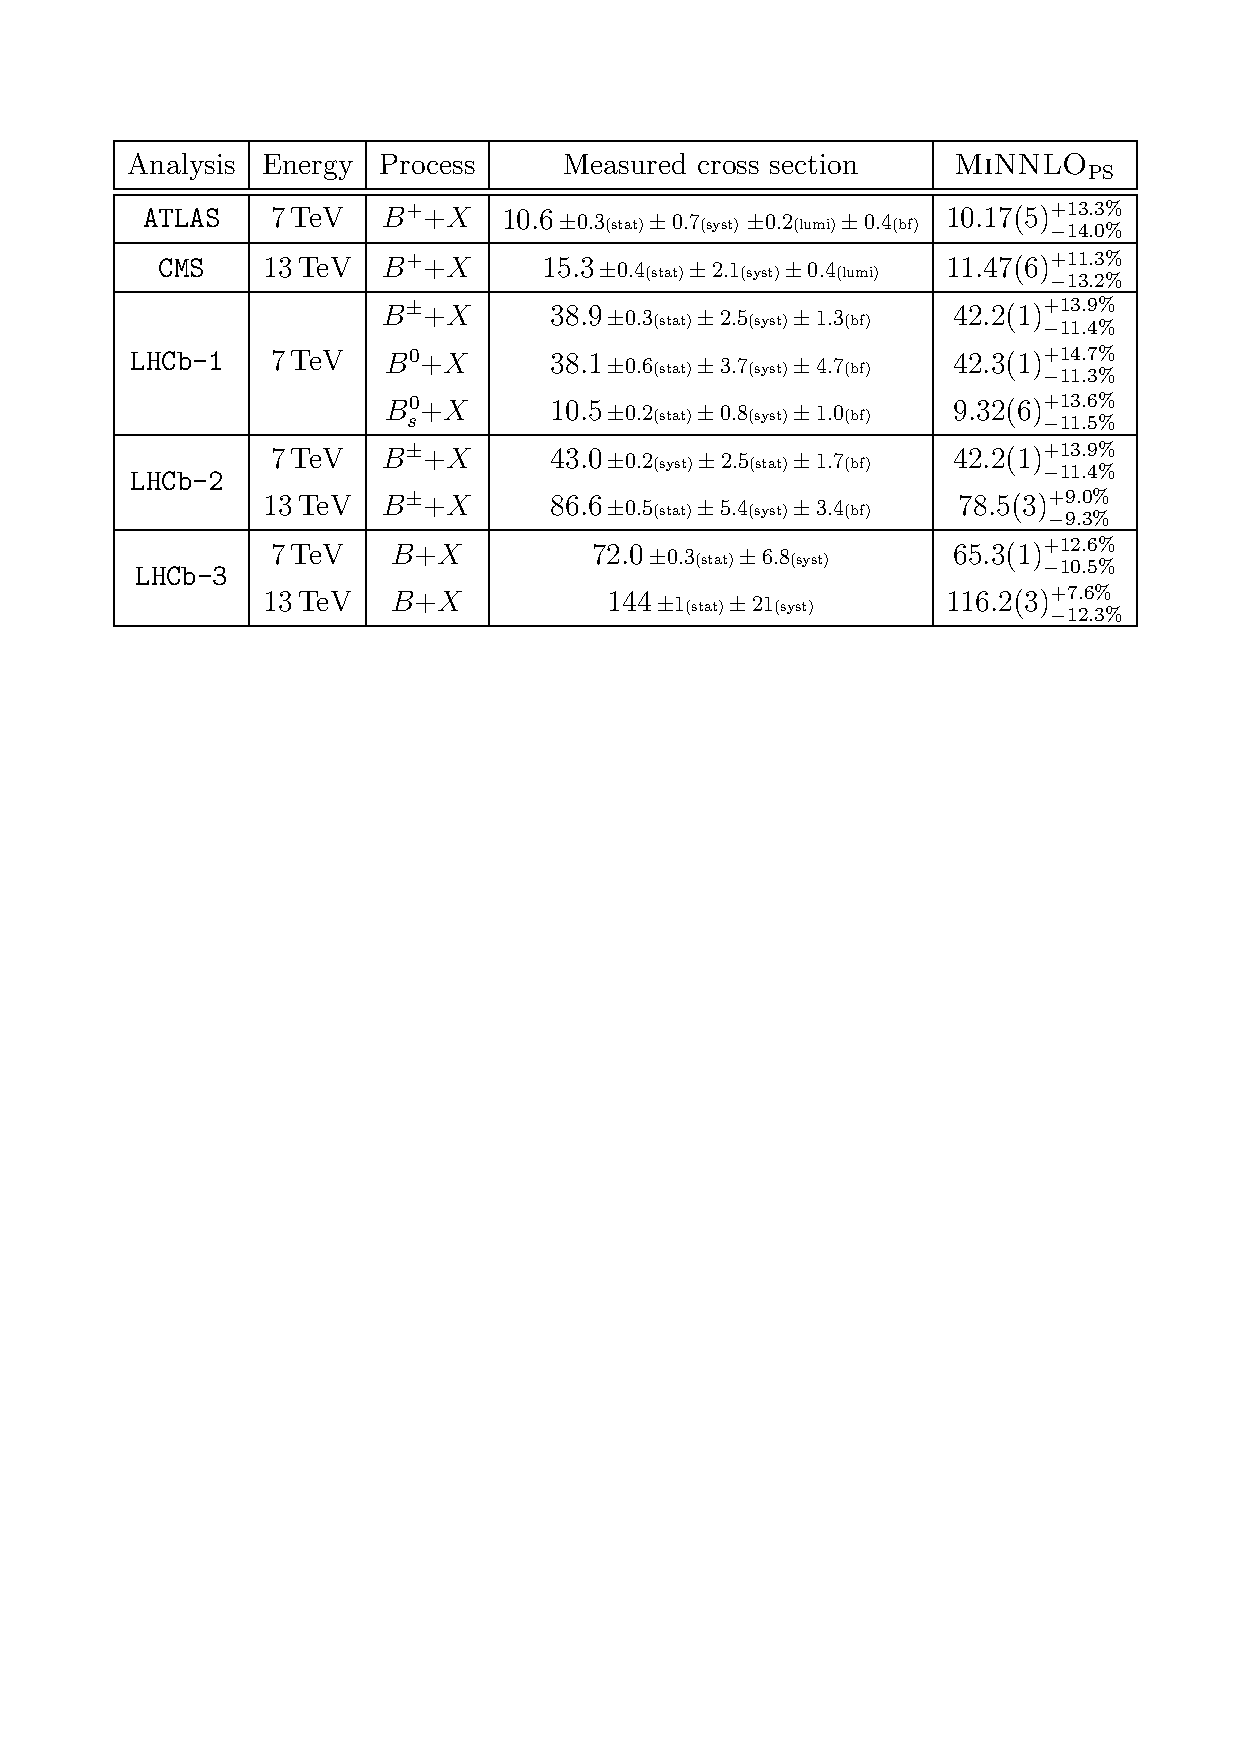
\includegraphics[width=1\linewidth]{plots/bb_table.pdf}
\caption{$B$-hadron cross sections for various experimental setups ($\mu$b).}
\label{tab:bb}
\end{center}
\end{table}

The $b\bar b$ \minnlo{} generator has been developed in \citere{Mazzitelli:2023znt} and employed for 
realistic predictions of $B$-hadron production in comparison to various LHC measurements.
By and large, a remarkable description of the measured cross sections is achieved, as reported in~\tab{tab:bb}. 
%see \tab{tab:bb} for instance. 
We are currently finalizing a second study where we 
consider $b$-jet observables using our $b\bar b$ \minnlo{} simulation.
%, as well as massless (and massive) NLO+PS dijet simulations. 
%
A preliminary comparison of our \minnlo{} predictions against ATLAS data is given in 
\fig{fig:bb}.
%
The developed generator also opens the possibility to study how the definition of the jet flavour (e.g. \citere{Gauld:2022lem}) can impact and limit the precision of the theory simulations.
This has potential implications for the choice of flavour tagging algorithms used by LHC experiments.
% and we find that the by far dominant effect 
%of the difference with to the standard $b$-tagging algorithms used by the experiments
%stems from the treatment of $g\to b\bar b$ splittings.
%


\begin{figure}[t]
\begin{center}
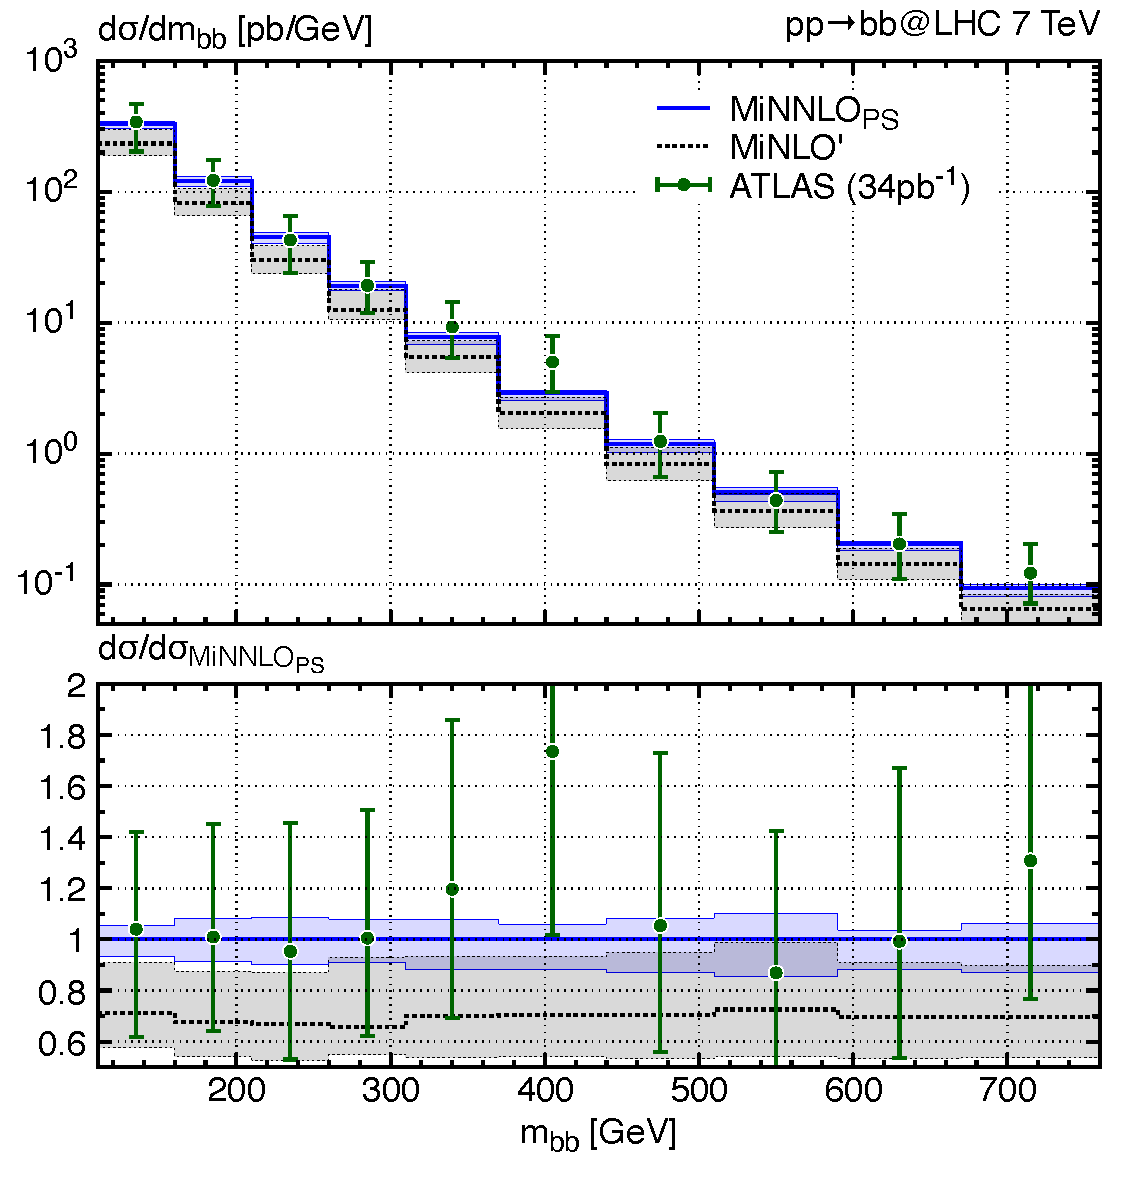
\includegraphics[width=0.95\linewidth]{plots/bjet_mbb.pdf}
\caption{Invariant-mass distribution of leading $b$-jets for \minnlo{} (blue), \minlo{} (grey).}
\label{fig:bb}
\end{center}
\end{figure}
%
\subsubsection[$D$-meson processes at NNLO+PS and prompt neutrino backgrounds]{\boldmath{$D$}-meson processes at NNLO+PS \mbox{and prompt neutrino backgrounds}}
\begin{Namen}
R. Gauld, T. Giani, A. Mahr, A. Ratti, M. Wiesemann, G. Zanderighi
\end{Namen}

Another important application of the developed \minnlo{} methology is to the production
of a charm-quark pair ($c\bar c$) in hadron--hadron collisions. 
%
Experimental studies of the production rates of charm production in $pp$, $pA$ and $AA$ collisions are carried out by the LHC experiments, and the interpretation of their data is relevant for our understanding of both nuclear and proton structure, as well as providing unique information on states of matter such as the quark gluon plasma.
%
%This process is relevant for all LHC experiments. 
%While this process also receives
%substantial attention by the current LHC experiments, additionally it plays a crucial role in 
%the envisaged forward-physics experiments, in particular FASER. ]
%
%Even more crucially, it is source of a major background to neutrino telescopes, such as ICECUBE, namely
%the atmospheric prompt neutrino flux.
%
Furthermore, charm hadron-hadron production is also relevant for neutrino telescopes, such as IceCube, as knowledge of the rate of the prompt atmospheric neutrino flux (induced by charm production in the atmosphere) is essential for studies of neutrinos of cosmic origin.
%
In all of these cases, the underlying mechanism is the production of charm quarks through the collision
of hadrons (either in a controlled collider environment or through cosmic rays interactions 
with the atmosphere), and the charm quarks then hadronize to $D$-mesons. In the case of atmospheric charm production, 
semi-leptonic decays then generate a flux of high energy neutrinos. 
%their further decay process highly energetic neutrinos are produced.

We have implemented a \minnlo{} generator for $c\bar c$ production to compute
$D$-meson cross sections at NNLO+PS. Moreover, we have begun to study 
the propagation of particles through the the atmosphere through cascade equation
based on the code Matrix Cascade Equations (MCEq) \cite{Fedynitch:2015zbe} to compute the prompt
atmospheric neutrino flux. In \fig{fig:neutrinoflux} the prompt atmospheric (electron) neutrino
flux is shown as a function of the neutrino energy comparing our LO and NLO+PS
inputs to the default ones of MCEq. As can be seen, the NLO corrections are substantial.
Moreover, the perturbative scale uncertainties (not shown here) are similarly large, 
jeopardizing the precision of the predictions for the neutrino flux. 
This is a severe limitation, which calls for the inclusion of higher-order corrections.
By upgrading these predictions with NNLO accuracy for $c\bar c$ production of 
our \minnlo{} generator we hope to significantly improve the estimation of the 
prompt atmospheric neutrino background in IceCube in terms of both accuracy and
precision.

\begin{figure}[b!]
\begin{center}
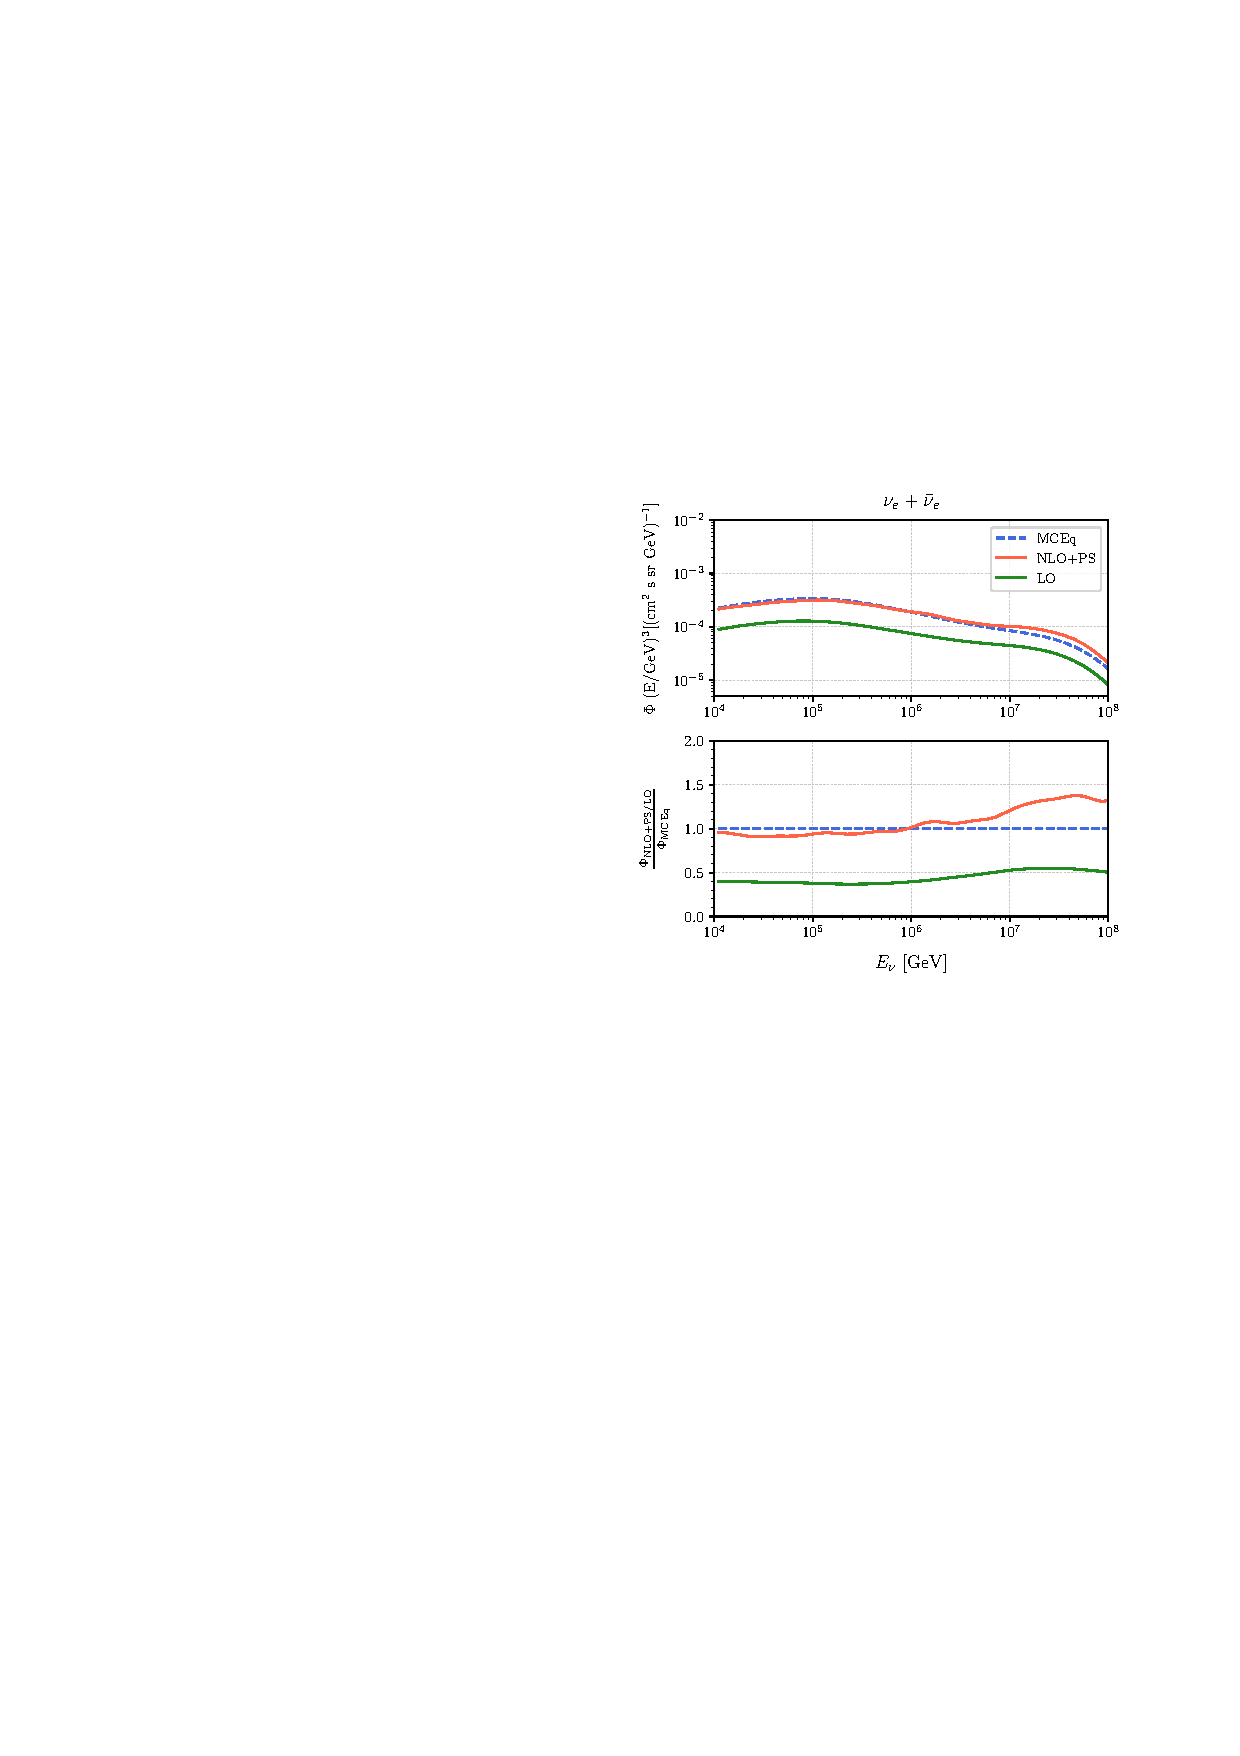
\includegraphics[width=0.95\linewidth]{plots/cc_neutrino_flux.pdf}
\caption{Prompt electron neutrino flux as a function of the neutrino energy.}
\label{fig:neutrinoflux}
\end{center}
\end{figure}

%
\subsubsection[\minnlo{} method for heavy-quark plus colour-singlet production and application to $b\bar{b}Z$ process]{\minnlo{} method for heavy-quark plus colour-singlet production and the \boldmath{$b\bar{b}Z$} process}
\begin{Namen}
M. Wiesemann
\end{Namen}
%
Just recently, we have derived the extension of the \minnlo{} formalism to deal with the production of a heavy quark pair and a colour singlet \cite{Mazzitelli:2024ura}.
It is based on the resummation formula for the transverse momentum of the final-state system as in previous \minnlo{} 
formulations. Although the resummation formula has the same structure as for a heavy quark pair, we had to correctly
account for the general kinematics of the final state, since the two heavy quarks are no longer back-to-back.

With this work, we have paved the way for a number of new NNLO+PS calculations, involving processes with two heavy quarks (top, bottom, charm) 
and one or more colour singlet bosons ($Z$, $W$, Higgs) including their decays. In fact, even the full off-shell process of top-quark pair production 
and decay belongs to that category. As a first application, we have considered the associated production of two bottom quarks and a $Z$ boson ($b\bar{b}Z$)
in the four-flavour scheme (4FS) \cite{Mazzitelli:2024ura}. With this calculation we have solved the long-standing tension between NLO 4FS predictions with data and with five-flavour scheme (5FS) predictions. 
As can be observed in \fig{fig:bbZ}, the NNLO corrections are substantial and are necessary to describe LHC data.

\begin{figure}[bh]
\begin{center}
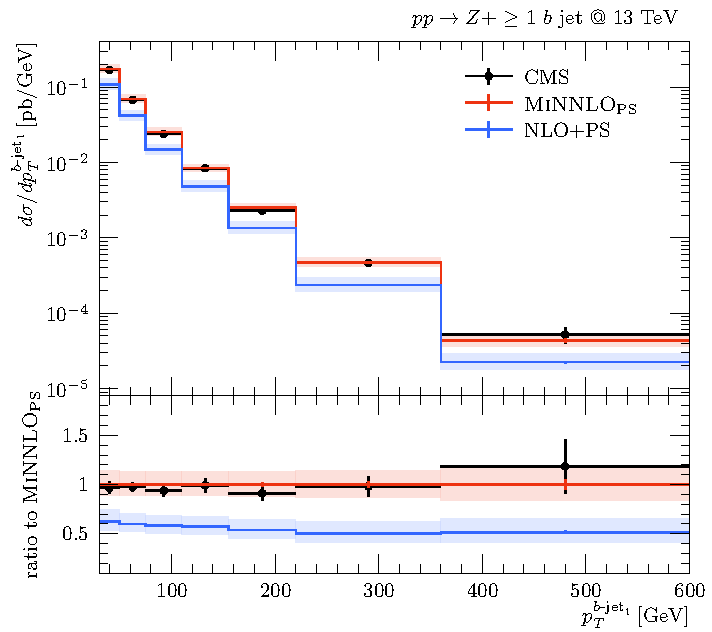
\includegraphics[width=0.95\linewidth]{plots/bbZ_ptbjet.pdf}
\caption{$b$-jet $p_T$ spectrum of \minnlo{} (red), NLO+PS (blue) and CMS data (black).}
\label{fig:bbZ}
\end{center}
\end{figure}


\subsubsection{Associated Higgs production with bottom quarks: a flavour-scheme study at NNLO+PS}
\begin{Namen}
C. Biello, R. Gauld, A. Sankar, M. Wiesemann, G. Zanderighi
\end{Namen}
Higgs production in association with bottom quarks (\bbH{}) is a rare production mode at the LHC, serving as an irreducible background in Higgs-pair searches and potentially gaining enhancement in BSM scenarios. 
Precise predictions of this process are important not only for experimental comparisons but also serve as a theoretical laboratory for studying heavy-flavour quark effects. 
In processes involving bottom quarks, predictions can be obtained using different approaches to mass effects. In the 5FS scheme, the bottom-quark component of the proton is perturbatively generated, enabling the resummation of large logarithmic contributions in the bottom mass. 
This approach treats the bottom quark as a massless parton, allowing for efficient high-order calculations. In~\citere{Biello:2024vdh}, we presented the first NNLO+PS simulation of this process within the massless scheme. For a more detailed description of bottom-quark kinematics, an alternative approach considers the production of massive bottom quarks in the hard scattering process, along with the Higgs boson, with the four lighter flavoures treated as massless (4FS). 
While computationally more demanding, this latter approach retains all mass effects order by order in perturbative QCD. Working in the \minnlo{} framework, which enables NNLO-accurate predictions for heavy-quark pair production in generic kinematics, we accessed the NNLO corrections in the massive scheme and matched them with a parton shower simulation~\citere{Biello:2024pgo}. 
Strong tensions between the predictions in either massless or massive schemes in \bbH{} were observed in the past (at lower perturbative orders), 
whereas a better agreement is found between the two NNLO+PS predictions, as shown in~\fig{phenofig:bbH}. 
The two schemes capture complementary aspects of bottom-quark dynamics. A generalised mass-variable flavour number scheme is desirable to achieve precise predictions across the full phase space. Using the method developed in~\citere{Gauld:2021zmq}, we are investigating the isolation of mass power corrections within the massive scheme, aiming to incorporate them into the massless prediction. This would allow us to retain the logarithmic resummation benefits of the massless scheme while systematically accounting for missing power corrections in the bottom quark mass.

\begin{figure}[phtb]
\begin{center}
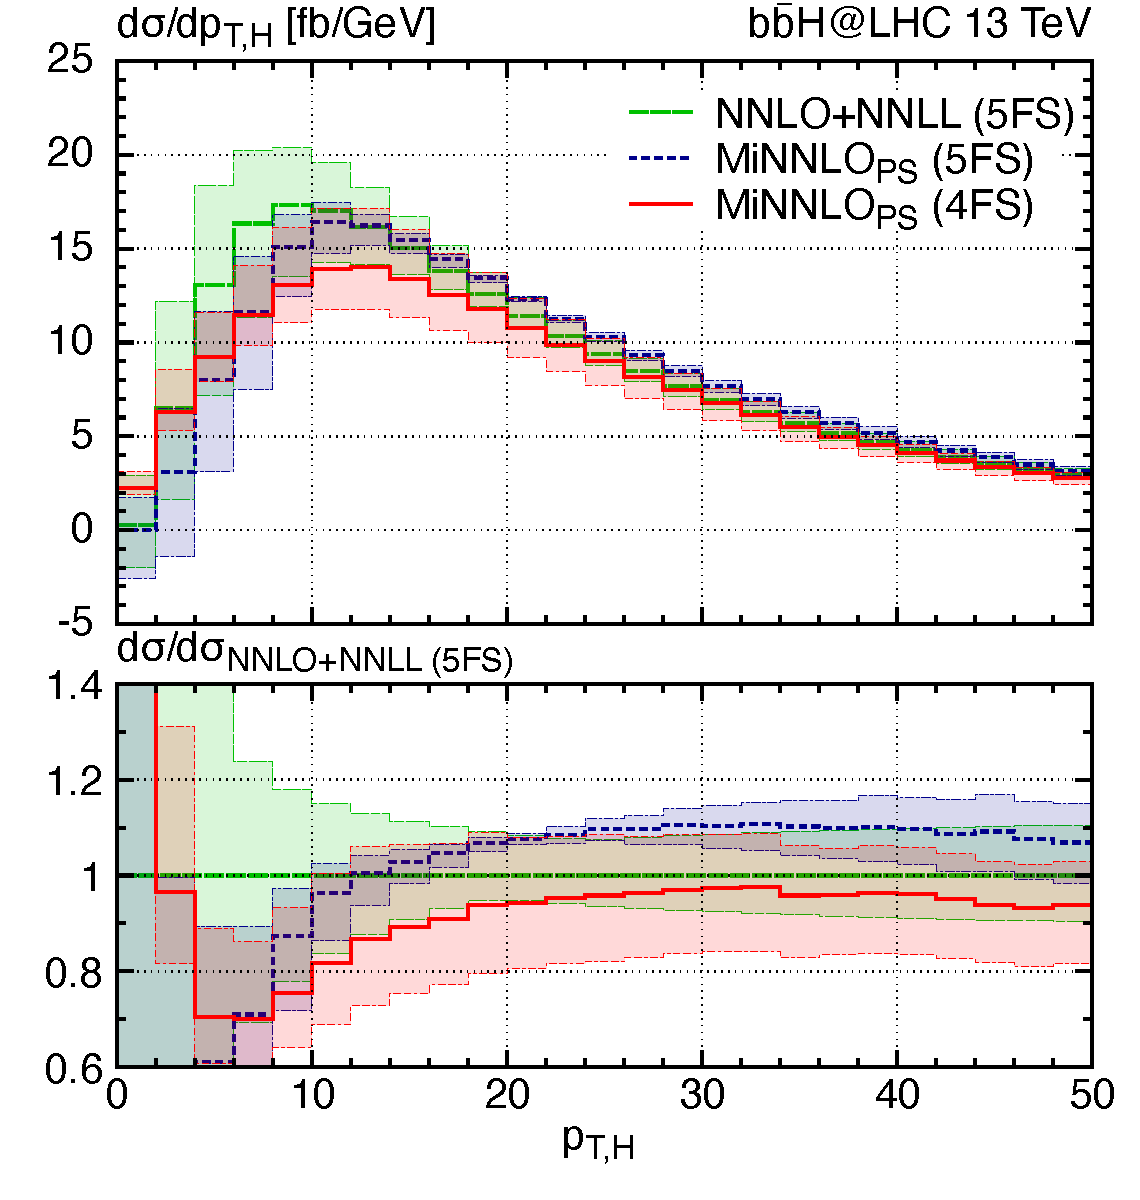
\includegraphics[width=0.95\linewidth]{plots/bbH__ptHspectrum.pdf}
\caption{Transverse spectrum of the Higgs boson produced via the bottom-quark Yukawa interaction at NNLO+PS in the massless (5FS, blue, dotted) and massive (4FS, red, solid) schemes~\cite{Biello:2024pgo}, with an NNLL+NNLO resummation result in the massless scheme (green, dashed).}
\label{phenofig:bbH}
\end{center}
\end{figure}
%
\subsubsection{Off-shell top-quark pair production at NNLO+PS}
\begin{Namen}
C. Biello, C. Signorile-Signorile, M. Wiesemann, G. Zanderighi
\end{Namen}
Given the experimental possibilities provided by the LHC to study the properties of the top quark through decay products, theoretical efforts are required to accurately describe off-shell effects in top-quark pair production. The current advancement of the \minnlo{} method enables the precise simulation of this process, including decay effects in the fully leptonic channel ($pp\rightarrow e^-\bar{\nu}_e\mu^+\nu_\mu b\bar b$). With six particles in the final state at leading order, this represents the highest multiplicity configuration we are currently investigating at NNLO+PS. Its complexity poses both computational and conceptual challenges: we address the high computational cost by improving the numerical efficiency of the code, while in the absence of an exact two-loop amplitude we investigate the development of reliable approximations.
% 
\subsubsection[\minnlo{} method for jet processes using $N$-jettiness]{\minnlo{} method for jet processes using \boldmath{$N$}-jettiness}
\begin{Namen}
M. Ebert, M. Wiesemann, G. Zanderighi, S. Zanoli
\end{Namen}
Despite processes involving light jets in the final state building a 
central class of LHC reactions, no NNLO+PS generators exist for any of them.
With the work of \citere{Ebert:2024zdj}, we have initiated the further extension of the \minnlo{} method by
formulating it in terms of the $N$-jettiness variable. This jet-resolution variable,
in principle, enables the treatment of any $N\ge 0$ jets in the final state within the 
NNLO+PS matching. In \citere{Ebert:2024zdj} we considered the case $N=0$, namely colour-singlet
production, and compared our new $0$-jettiness predictions with the original \minnlo{}
ones using the transverse momentum of the colour singlet.
Moreover, we discussed the $N=1$ case, applicable to colour singlet
plus jet production, by deriving the \minnlo{} formalism for $1$-jettiness.
%
\subsubsection{Inclusion of electroweak corrections in \minnlo{}}
\begin{Namen}
G. Pelliccioli, M. Wiesemann, G. Zanderighi, S. Zanoli
\end{Namen}

\begin{figure}[b!]
\begin{center}
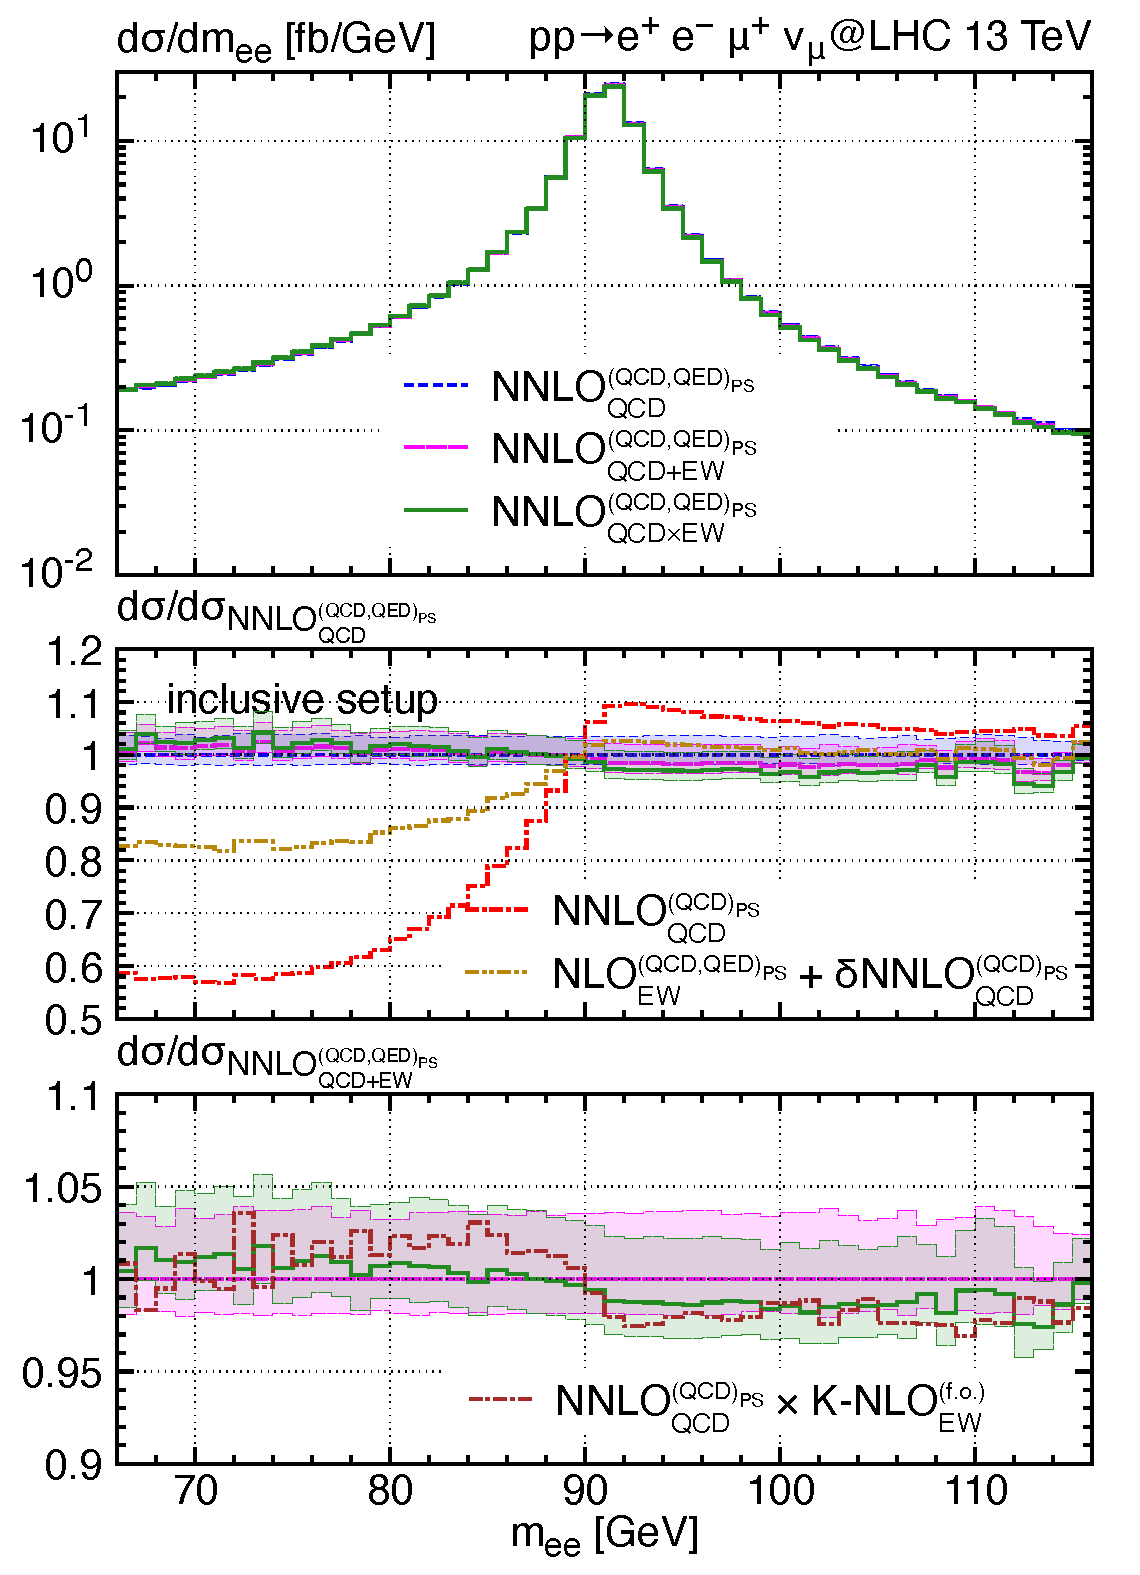
\includegraphics[width=0.95\linewidth]{plots/MiNNLO_EW_WZ_mZ.pdf}
\caption{Dilepton mass in $WZ$ process.}
\label{fig:WZ}
\end{center}
\end{figure}

Although, by and large, 
QCD perturbation theory provides the dominant corrections at hadron 
colliders due to the size of the strong coupling at the relevant energies, 
electroweak (EW) effects are indispensable for the precision programme of the LHC.
In certain phase-space regions EW corrections can even become dominant. This is the case
when observables become sensitive to photon radiation, e.g. for invariant-mass 
distribution of a group of leptons, or in the high-energy tails of kinematical distributions,
where EW Sudakov logarithms yield substantial effects.

Given that \minnlo{} provides the most accurate event simulations in 
perturbative QCD to date, the inclusion of EW effects in these predictions
is an important extension. In \citere{Lindert:2022qdd}, we developed a \minnlo{} NNLO+PS generator 
as well as a POWHEG NLO+PS  generator including QCD and EW corrections 
for $WZ$ production. We then studied, different approaches to combine the
QCD NNLO+PS predictions with the EW NLO+PS predictions using additive 
and multiplicative matching schemes as well as different treatments of the 
QCD and QED radiation in the parton showers.
As an example, \fig{fig:WZ} shows the crucial importance of photon radiation
to describe the Z-boson line shape (cf. difference with 
red dash-dotted line in first ratio inset, which is the pure QCD prediction).

Currently, we are working towards a more sophisticated inclusion of EW effects 
by accounting for NLO EW corrections for $WZ+jet$ production
directly within the \minnlo{} formulae. We then aim to supplement the all-order treatment 
with QED effects to reach NLO EW accuracy for inclusive $WZ$ observables without
extra jets. This approach is currently developed and tested for the Drell-Yan process.


\subsubsection{Polarized NLO+PS predictions and quantum info}
\begin{Namen}
G. Pelliccioli, G. Zanderighi
\end{Namen}
%

Polarised amplitudes are interesting as they can exhibit a stronger
sensitivity to new physics.
%
Starting from recent developments in polarised-boson simulation based
on the helicity selection at the amplitude level,
ref.~\cite{Pelliccioli:2023zpd} presents a calcualtion and simulation
of inclusive diboson processes (WZ, ZZ and WW). A phenomenological
analysis in realistic LHC setups, as well as a comparison with recent
ATLAS measurements, are presented.

Motivated by the growing interest in accessing the spin structure of
multi-boson processes and in measuring quantum entanglement at high
energies, ref.~\cite{Grossi:2024jae} studies polarisation and
spin-correlation coefficients in di-boson systems. It is shown that
higher-order corrections of QCD and electroweak type, off-shell
modelling, and realistic effects such as fiducial selections and
neutrino reconstruction are unavoidable to properly determine such
coefficients, and consequently to provide a sound interpretation of
observables sensitive to quantum entanglement and Bell-inequality
violation. These findings are based on a detailed phenomenological
analysis of boson pairs at the LHC, either in inclusive electroweak
production or coming from Higgs-boson decays.

\printbibliography[heading=subbibliography]
\end{refsection}

%%%%%%%%%%%%%%%%%%%%%%%%%%%%%%%%%%%%%%%%%%%%%%%%%%%%%%%%%%%%%%%%%%%%%%
\subsection{Precision Higgs physics at the Large Hadron Collider}
%%%%%%%%%%%%%%%%%%%%%%%%%%%%%%%%%%%%%%%%%%%%%%%%%%%%%%%%%%%%%%%%%%%%%%
\begin{refsection}
With the discovery of the Higgs boson in 2012, CERN's Large Hadron Collider has made a 
historic contribution to particle physics. One of the major goals of the physics programme
of the LHC since its discovery is the precise determination of the properties of the Higgs
particles, including its mass and spin, its couplings to other particles, production and decay
rates. To this end, higher-order computations of Higgs reactions at the LHC are indispensable
to reach the most accurate determination of these quantities.

Within our group we have been pushing the precision of Higgs-boson production and decay
processes, at the level of both fixed-order calculations and fully exclusive event simulations,
since many years. 


\subsubsection{Quark-mass effects in Higgs production at NNLO}
\begin{Namen}
M. Niggetiedt
\end{Namen}
%

Gluon fusion is the predominant channel for the production of a Higgs boson at the LHC. This makes a firm understanding of the process and corresponding observables mandatory for current and future precision Higgs physics. Enormous efforts have been devoted to the precise theoretical description of the total inclusive gluon fusion cross section. It is important to emphasize that in the Standard Model the Higgs boson is the only particle featuring Yukawa interactions with fermions. Therefore, minimizing the associated theory uncertainties is of paramount importance as theory predictions for Higgs observables have a direct impact on the extraction of couplings and masses from experimental measurements.

A comprehensive analysis of the gluon fusion cross section by the LHC Higgs Working Group identified different sources of theory uncertainty which sum up to roughly $6\%$ uncertainty. About one third of this uncertainty is attributed to missing quark-mass effects at NNLO in QCD: a lack of exact knowledge of top quark and bottom quark mass effects at the cross-section level.

An exact description of top-quark mass effects has been previously presented in~\citere{Czakon:2021yub} while the role of bottom-quark-mass effects was unknown. Although, mass effects of the lighter quark flavors are suppressed due to the Yukawa coupling to the Higgs boson, interference effects between the top and bottom quark have been estimated to be of the order of $1\%$. 

To overcome this, knowledge of the two-loop amplitudes for the H+jet process and three-loop amplitude for the $gg \to H$ amplitude including bottom-quark-mass effects have been obtained~\citere{Czakon:2023kqm,Niggetiedt:2023uyk}. In a first study \cite{Czakon:2023kqm} top-bottom interference contribution to the fully inclusive Higgs production cross section at NNLO in QCD has been evaluated. The effect of the interference turned out to be $-1.99(1)^{+0.30}_{-0.15}$~pb at $13\,\mathrm{TeV}$ as a result of non-trivial cancellations between the pure NLO and NNLO corrections. In particular, the $\mathcal{O}(\alpha_s^4)$ corrections amount to $0.43$~pb almost completely compensating the NLO shift.

Further studies on the dependence of the renormalisation scheme as well as the impact of quark mass effects on differential distributions has been carried out in~\citere{Czakon:2024ywb}. The differential results indicate sensitivity to the choice of bottom-quark mass renormalisation scheme in certain kinematic regions, and a corresponding NNLO calculation matched to parton shower is work in progress to further investigate such effects.

%We have put forward the exact description of the previously unknown quark-mass effects at NNLO QCD in \cite{Czakon:2021yub} where the top-quark mass effects on the total Higgs production cross section have been addressed. Our analysis revealed that finite top-quark mass effects beyond the well-established rescaled heavy-top limit give rise to a small shift of $-0.32\%$ on the total cross section at $13\,\mathrm{TeV}$ and $-0.16\%$ at $8\,\mathrm{TeV}$ \cite{Czakon:2021yub}. This result confirms and at the same time eliminates the commonly accepted uncertainty estimate arising from the lack of knowledge of top-quark mass effects.

%For the determination of interference effects the efficient evaluation of two-loop H+jet amplitudes with a massive bottom flavor is required. To achieve this, and building upon~\citere{Czakon:2021yub}, techniques have been developed to overcome numerical instabilities when solving the relevant Feynman integrals even at the edges of the physical phase space.

%Additionally, when considering NNLO QCD corrections with two massive quark flavors, a new class of Feynman diagrams emerges in the three-loop virtual corrections to the $gg \to H$ amplitude. We have derived deep asymptotic expansions of the corresponding amplitude which converge in the parameter space relevant for the assessment of interference effects between the top and the bottom quark and numerically sampled the domains not accessible with the expansions \cite{Niggetiedt:2023uyk}.

%The new two-loop amplitudes for the H+jet process with full quark-mass dependence have been combined with the aforementioned three-loop double-virtual corrections and the one-loop double-real corrections. In a first study \cite{Czakon:2023kqm} top-bottom interference contribution to the fully inclusive Higgs production cross section at NNLO in QCD has been evaluated. The effect of the interference turned out to be $-1.99(1)^{+0.30}_{-0.15}$~pb at $13\,\mathrm{TeV}$ as a result of non-trivial cancellations between the pure NLO and NNLO corrections. In particular, the $\mathcal{O}(\alpha_s^4)$ corrections amount to $0.43$~pb almost completely compensating the NLO shift.

% RG new version
%Further studies on the dependence of the renormalisation scheme as well as the impact of quark mass effects on differential distributions has been carried out in~\citere{Czakon:2024ywb}. The differential results indicate sensitivity to the choice of bottom-quark mass renormalisation scheme in certain kinematic regions, and a corresponding NNLO calculation matched to parton shower is work in progress to further investigate such effects.

%We note that the aforementioned numbers have been obtained with quark masses renormalized in the on-shell scheme and employing the 5-flavor scheme. To conclusively determine the effect of the top-bottom interference on the gluon-fusion process, we have performed a thorough analysis of the total cross section and more differential quantities making use of different renormalization and flavor schemes \cite{Czakon:2024ywb}. We have found excellent agreement between the 5-flavor and 4-flavor scheme for the interference contribution, justifying the treatment of the bottom-quark mass in the 5-flavor scheme. Our computation in two different renormalization schemes showed that renormalizing the bottom-quark mass in the $\overline{\mathrm{MS}}$ scheme results in significantly smaller scale uncertainties and displays a better perturbative convergence. The renormalization of the top-quark mass on the other hand does not impact the cross section significantly.

%Furthermore, we have provided differential distributions for the Higgs rapidity as well as for the $p_T$ of the Higgs boson. The differential results revealed that the sensitivity of the cross section on the choice of renormalization scheme for the bottom-quark mass originates from the low-$p_T$ region where also non-perturbative effects must be taken into account. The corresponding NNLO calculation matched to parton shower is work in progress and particularly aims for a precise description of the light-quark mass effects, and we reckon that it will be a useful addition to ongoing and future experimental analyses.
%

\subsubsection{Full top-mass dependence in Higgs production at NNLO+PS}
\begin{Namen}
M. Niggetiedt, M. Wiesemann
\end{Namen}

\begin{figure}[h!]
\begin{center}
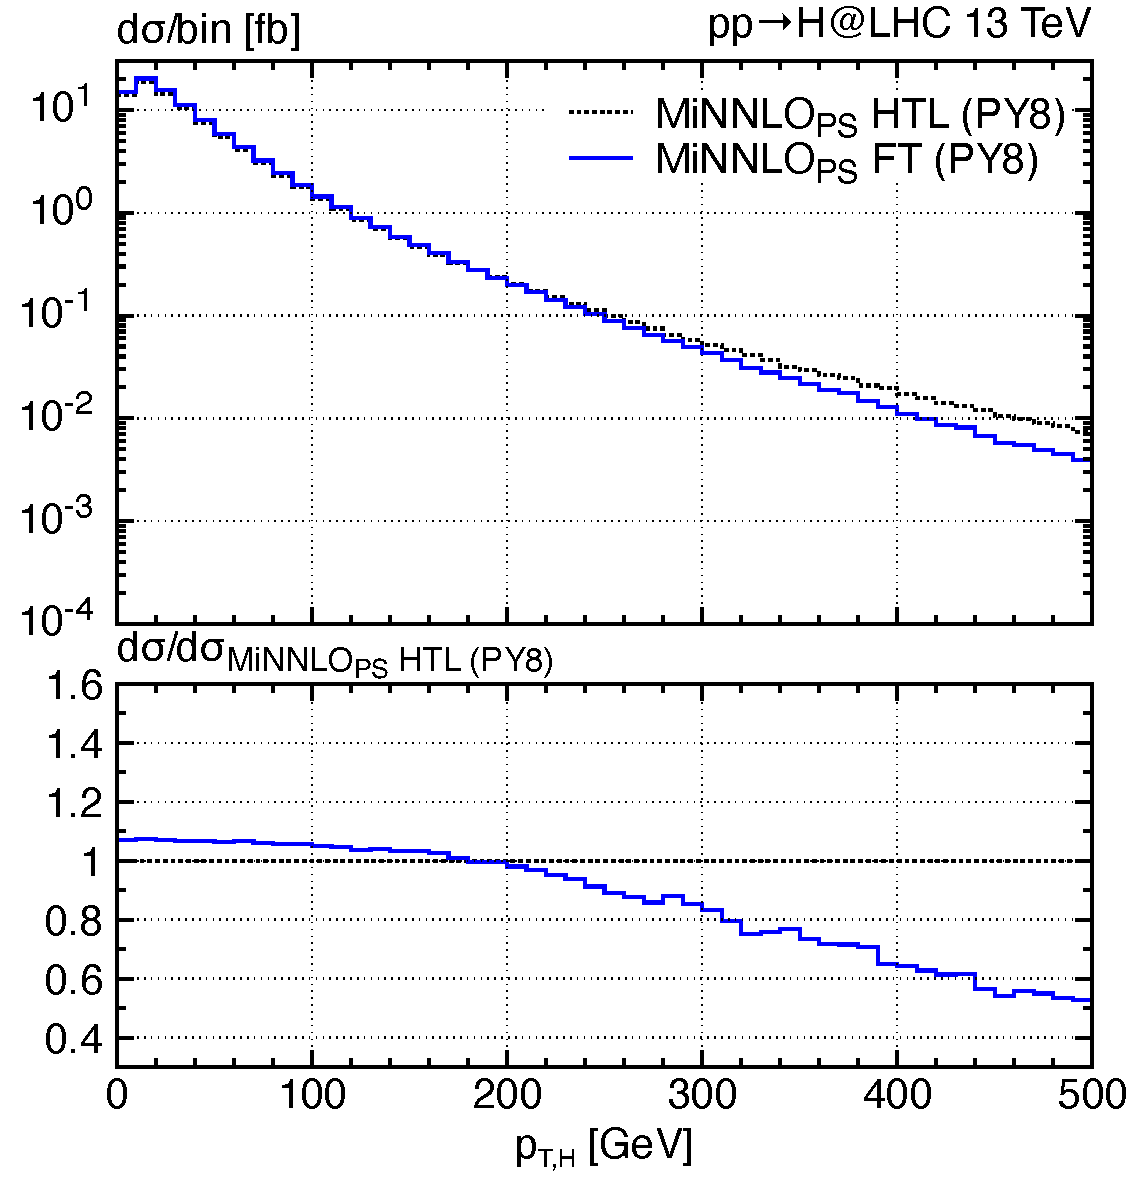
\includegraphics[width=0.95\linewidth]{plots/ptH_diphotons_mass_effect.pdf}
\caption{Top-mass effect in Higgs $p_T$ spectrum.}
\label{fig:topmass_Higgs_pT}
\end{center}
\end{figure}
%
Based on the calculation of the inclusive NNLO cross section in the full theory
including the complete top-mass effects,
we have developed the first (and so far only) 
NNLO+PS generator for the loop-induced 
Higgs production process in gluon fusion in the full theory using 
the \minnlo{} method in \citere{Niggetiedt:2024nmp}. Figure\,\ref{fig:topmass_Higgs_pT} shows
the crucial importance of top-mass effect in differential Higgs production
at NNLO+PS at the example of the Higgs transverse-momentum ($p_T$)
spectrum by comparing the full theory result (blue solid) against
the approximation of an infinitely heavy top quark (black, dashed).

In \citere{Niggetiedt:2024nmp} we have also quantified the high quality of relevant approximations 
of the top-mass effects at NNLO, which were feasible before, in comparison to our 
novel full-theory results. These results will be useful to provide well-motivated 
approximations of top-mass effects beyond NNLO. Currently, we are extending 
our \minnlo{} calculation by the complete dependence on light-quark mass 
effects (bottom and charm) up to NNLO.

%
\subsubsection{VBF $H\rightarrow b\bar{b}$ production}
\begin{Namen}
A. Behring, G. Zanderighi
\end{Namen}
Higgs production in vector boson fusion (VBF) is the second most common
production channel at the LHC. This explains the considerable interest from
both theorists and experimentalists in precise descriptions of this process.
The Higgs also decays predominantly to a pair of $b$ quarks, making the
combination of VBF with the $H \to b\bar{b}$ decay channel even more
interesting.

Following developments where the production \cite{Asteriadis:2021gpd} and decay
\cite{Behring:2019oci} have been studied separately at NNLO in QCD, we combined
these descriptions in Ref.~\cite{Asteriadis:2024nbg} in the narrow-width
approximation.
%
It turned out that the NNLO corrections for the fiducial cross-section at NNLO
show only slow perturbative convergence. 
%This came as a surprise since neither
%the production nor the decay, when considered separately, show such a
%behaviour. In particular, this raises concerns whether a description at NNLO in
%QCD is sufficient for accurate predictions of this process.
In Ref.~\cite{Asteriadis:2024nbg} we managed to trace this back to an interplay
of additional radiation from the Higgs decay at higher perturbative orders with
the definition of the fiducial cuts. These cuts (inspired by an analogous ATLAS
analysis), include a cut on the transverse momentum of the subleading $b$ jet
of $p_{T,b_2} \geq 65\,\mathrm{GeV}$. This happens to place the cut at a point
where the transverse momentum spectrum is steeply falling, and therefore makes
observables with this cut highly susceptible to additional radiation added by
higher-order corrections.

This observation has led us to ask the question whether effects from this additional radiation could already be captured by a parton shower description
of the decay process. % In particular it is interesting whether a NNLO description matched to a parton shower shows better perturbative convergence.
%
Given the expertise with parton-shower-matched calculation in the group at MPP, it was natural to join forces and combine the NNLO+PS calculation for $H \to b\bar{b}$ decays from Ref.~\cite{Bizon:2019tfo} with the NNLO description for VBF from Ref.~\cite{Asteriadis:2021gpd}. This project is currently ongoing.

\subsubsection{Higgs Boson Production in Association with a Top-Antitop Quark at NNLO}
\begin{Namen}
 J. Mazzitelli 
\end{Namen}

The associated production of a Higgs boson with a top-antitop quark pair is a crucial process at the LHC since it allows for a direct measurement of the top-quark Yukawa coupling. Ref.~\cite{Catani:2022mfv} presents the computation of the radiative corrections to this process at NNLO. This is the very first computation for a $2 \to 3$  process with massive colored particles at this perturbative order. A soft Higgs boson approximation for loop amplitudes is developped, which enables one to reliably quantify the impact of the yet unknown two-loop contribution. It is foudn that at LHC collisions at the center-of-mass energy $s=13$\,TeV, the NNLO corrections increase the NLO result for the total cross section by about 4\% and lead to a significant reduction of perturbative uncertainties.

\subsubsection{Di-Higgs production at NNLO+PS}
\begin{Namen}
F. Garosi, S. Kumar, M. Wiesemann, G. Zanderighi
\end{Namen}
Our best opportunity to access the Higgs potential at the LHC is through the measurement
of a pair of Higgs bosons. Di-Higgs production is directly sensitive to the trilinear Higgs coupling,
allowing us to put bounds on its value and possibly even measuring its size with the full HL-LHC data.

Since di-Higgs production is a loop-induced $2\to 2$ process the computation of higher-order 
corrections is quite cumbersome, and so far limited to NLO in the full theory. However, by combining
the full-theory NLO predictions with calculations in the heavy-top limit, it is possible to obtain 
meaningful approximations of the NNLO cross section. Following this idea, we are currently 
implementing a new NNLO+PS generator for Higgs-pair production using the \minnlo{} method.

%
\subsubsection{Beyond the leading-power}
\begin{Namen}
A. Sankar
\end{Namen}
%
The fixed-order description of Higgs boson production at the LHC often receives large numerical contributions from kinematic regions (close to threshold) involving soft logarithmic enhancements. The impact of next-to-soft --- commonly referred to as next-to-leading power (NLP) terms --- can also lead to large numerical effects.
%
The impact of such terms has been computed via all-order NLP resummed corrections an applied to the case of the SM Higgs boson~\citere{Das:2024pac} as well as a (BSM) pseudo-scalar Higgs boson~\citere{Ravindran:2023qae}. In both cases, extensive phenomenological analyses to study the impact of NLP resummation on Higgs production at the LHC have been presented.

%I worked on the study of next-to-soft threshold effects—commonly referred to as next-to-leading power (NLP) terms—in the context of scalar and pseudo-scalar Higgs production, with the results published in~\cite{Das:2024pac} and~\cite{Ravindran:2023qae}, respectively. In these works, we computed all-order NLP resummed corrections within perturbative QCD and performed extensive phenomenological analyses to study the impact of NLP resummation on Higgs production at the LHC.

\printbibliography[heading=subbibliography]
\end{refsection}


\subsection{Development of methods for fixed-order calculations and their applications}
\begin{refsection}

Many of the phenomenological results discussed in the previous sections, such as those based on the \minnlo{} method, have relied on the availability of either fixed-order calculations or the perturbative ingredients of NNLO QCD calculations.
%
In some of these cases, the precision of the available data from experiment already places more strong demands on the theory community.
%
The continued development of theoretical tools and methods is therefore critical to improve the modelling of the theory predictions. This remains an active research activity of our group, for example: towards automation of or going beyond NNLO QCD, the inclusion of quark mass effects, the efficient evaluation of Feynman integrals.

\subsubsection{Infrared subtraction at NNLO in perturbative QCD}
\begin{Namen}
G. Pelliccioli, A. Ratti, C. Signorile-Signorile
\end{Namen}
%
To achieve reliable theoretical predictions for key QCD processes, it is essential to explore higher orders in perturbation theory. This requires dealing with infrared (IR) singularities that arise from both virtual and real corrections. While efficient and process-independent methods for handling IR singularities at next-to-leading order (NLO) in QCD were developed decades ago, a fully general solution at next-to-next-to-leading order (NNLO) remains elusive, despite significant progress over the past twenty years.
As a result, numerous NNLO subtraction schemes continue to be developed and refined. In Ref.~\cite{Bertolotti:2022aih}, the \emph{local analytic sector subtraction} method was employed to demonstrate the cancellation of IR singularities for arbitrary processes at $e^+e^-$ colliders. This approach yields compact and fully analytic expressions, making it well-suited for direct numerical implementation. To date, it remains the only fully local and analytic subtraction scheme capable of achieving this level of generality for lepton scattering at NNLO in QCD.
More recently, Ref.~\cite{Magnea:2024jqg} marked the first steps toward extending this framework to N${}^3$LO, along with some complementary studies based on the factorisation properties of gauge amplitudes that can lead to interesting insights on the general organisation of subtraction schemes at all orders in perturbation theory.
In parallel, addressing the growing demand for precision predictions in multi-parton processes at hadron colliders, the \emph{nested soft-collinear subtraction} scheme has been revisited to cope with $pp$ scatterings into arbitrary number of coloured and colourless partons. Notably, in Ref.\cite{Devoto:2023rpv} and~\cite{Devoto:2025kin}, 
a novel formulation of the \emph{nested soft-collinear subtraction} was presented. 
A key feature of this revised approach is the identification of iterative structures within the subtraction terms,
enabling significant simplifications in the intermediate steps of the calculations and ameliorating the physical transparency of the results. 
Although not yet fully general, the approach outlined in these references represents an important milestone toward obtaining finite remainders of the integrated subtraction terms for generic hadron collider processes within the nested soft-collinear subtraction scheme.


%
\subsubsection{Four-loop renormalisation of pseudoscalar operators}
\begin{Namen}
M. Niggetiedt
\end{Namen}
%
The treatment of the chiral matrix $\gamma_5$ in loop diagrams within dimensional regularization is a well-known technical challenge. Non-anticommuting $\gamma_5$ schemes are commonly used due to their technical ease and the availability of results for necessary renormalization constants. However, the use of a non-anticommuting $\gamma_5$ scheme may break certain symmetry properties of matrix elements or Green's functions giving rise to anomalous terms at the bare level. In order to recover the broken symmetry properties, $\gamma_5$-related symmetry-restoration renormalizations must be applied. 

In our study~\cite{Chen:2024cvu}, we have for the first time calculated the renormalization constant for a pseudoscalar operator regularized with a non-anticommuting $\gamma_5$ in dimensional regularization up to four-loop order in QCD. We have conducted a decomposition of the renormalization constant of the pseudoscalar operator, in order to separate explicitly the component that arises solely from $\gamma_5$-related symmetry-restoration. This facilitates the transformation to other (non-$\overline{\mathrm{MS}}$) renormalization schemes. Exploiting the renormalization-group invariance of the appropriately defined renormalization constant for this operator, we have been able to obtain the corresponding $\overline{\mathrm{MS}}$ factor at five-loop order in QCD. 
%
\subsubsection{Soft function at N3LO}
\begin{Namen}
M. Delto, C. Wang
\end{Namen}
%
In the coming high luminosity LHC era, describing the highly precise differential cross-sections requires us to understand the intricate infrared structures of QCD at even higher perturbative order.
In order to produce meaningful cross-sections, we need to correctly subtract the spurious infrared divergences before integrating the amplitude over the phase space.
$N$-jettiness slicing is one of many ways to resolve this problem, but it is not available at $\text{N}^{3}\text{LO}$ due to the absence of the soft function calculation.
In~\cite{Baranowski:2024ene,Baranowski:2024vxg,Baranowski:2024ysi}, we completed the calculation of the last missing ingredient of the zero-jettiness slicing method for color-singlet production at $\text{N}^{3}\text{LO}$, marking our first step towards the $N$-jettiness slicing method for general colorful final states.
Along the way, we developed several new computational techniques, such as the extended reverse unitarity method and the integral filtering method, which may find wider application in the field of precision calculation.
%
\subsubsection{Reclassifying Feynman Integrals as Special Functions}
\begin{Namen}
C. Wang
\end{Namen}
%
The Feynman integral is the central object in the perturbation theory of quantum field theory, and its evaluation is also one of the main sources of difficulties in our quest for even more precise theory predictions.
Intriguingly, various kinds of special functions in mathematics appear naturally in the computation of Feynman integrals.
In~\cite{Liu:2023jkr}, we proposed a recipe for efficiently evaluating Feynman integrals through the auxiliary mass flow method and differential equations in the kinematic variable space.
The efficient evaluation method available to Feynman integrals may also serve as a way of exploring the space of special functions.
%
%
\subsubsection{The $Q_{1,2}$--$Q_7$ interference contributions to $b \to s \gamma$ at ${\mathcal{O}}(\alpha_s^2)$ for the physical value of $m_c$}
\begin{Namen}
M. Niggetiedt
\end{Namen}
%
Rare $B$-meson decays provide important constraints on various BSM scenarios. Of particular interest in this context is the inclusive radiative decay $\bar{B}\to X_s\gamma$ which is currently measured with $5\%$ accuracy. %\cite{HeavyFlavorAveragingGroup:2022wzx,ParticleDataGroup:2022pth}. 
For $E_\gamma > 1.6 \,\mathrm{GeV}$, the $\bar{B}\to X_s\gamma$ decay rate is well approximated by the perturbative decay $b\to X_s^p\gamma$ with $X_s^p = s,sg,sgg,sq\bar{q},\ldots$ as partonic final states. 
%
In order to match the experimental accuracy, NLO electroweak as well as NNLO QCD (${\mathcal{O}}(\alpha_s^2)$) corrections need to be considered. In previous studies, some of the important NNLO QCD corrections that depend on the mass of the charm quark have only been addressed in the unphysical limit $m_c \gg m_b$ \cite{Misiak:2010sk}, or for a massless charm quark \cite{Czakon:2015exa}. The approximate treatment of charm-quark mass effects induces $3\%$ uncertainty on top of the $3\%$ uncertainty due to missing higher orders and $2.5\%$ due to input parameters and non-perturbative effects. 
%
While currently, experimental measurements and theory prediction are in agreement, the ultimate Bell II luminosity will allow for high-statistics measurements pushing the accuracy below $5\%$. This necessitates the elimination of uncertainties due to charm-quark mass effects in theory. 
%
To this end, we have computed all four-loop Feynman diagrams for the $b \to s \gamma$ transition with massive bottom and charm quarks in the framework of reverse unitarity. Thereby, the calculation has been separated into the evaluation of partial amplitudes with two, three, and four cut propagators. The most challenging contribution involving two cut propagators has been the subject of our work \cite{Czaja:2023ren}. 
%To deal with the high complexity of the underlying Feynman integrals, we have developed a semi-analytical technique based on differential equations, which allowed us to determine the desired amplitudes at high-precision. 
%
Our study constitutes a major step towards the full result for the $b \to s \gamma$ decay rate taking into account the exact charm-quark mass dependence at NNLO QCD. Meanwhile, the calculation of contributions with three and four cut propagators has been accomplished and the cancellation of UV and IR divergences when combined with the published results \cite{Czaja:2023ren} has been observed. A complete analysis including contributions from bremsstrahlung is currently in preparation. 
%

%
\subsubsection{Z+c-jet at NNLO QCD}
\begin{Namen}
R. Gauld
\end{Namen}
%
Another avenue of development is fixed-order calculations which take into account the full flavour information of scattering processes.
Such a development was required for the computation of the process $pp \to Z + c-{\rm~jet}$, as presented in~\citere{Gauld:2023zlv}. 
%
This computation furthermore incorporated charm quark mass effects beyond the leading-power, which was achieved combining both massive and massless approaches to describe the scattering process.
%
These developments led to substantial improvements in the precision of the theory calculation. At the same time, open questions about the role of multiple-particle-interactions and the definition of jet-flavour in experimental analyses were also raised in this work.


\subsubsection{Top-mass renormalization in ttbar @ NNLO}
\begin{Namen}
J. Mazzitelli
\end{Namen}
The ambiguity in the choice of a renormalization scheme and scale for
the top-quark mass leads to an important source of theoretical
uncertainty in the calculation of the Higgs boson production cross
section via gluon fusion.  Ref.~\cite{Mazzitelli:2022scc}, presents a
study of the uncertainties related to the top-quark mass definition up
to next-to-next-to-leading order (NNLO) in QCD.  NNLO predictions for
off-shell Higgs boson production in the soft-virtual approximation
renormalizing the top-quark mass within both the on-shell (OS) and the
MS schemes are presented. The study shows that the differences between
the two schemes are sizeable, but the difference is largely reduced
when increasing the order of the perturbative expansion. This work
also demonstrated explicitly that the convergence of the perturbative
series in the MS scheme is much better than in the OS one.
%
\printbibliography[heading=subbibliography]
\end{refsection}


%%%%%%%%%%%%%%%%%%%%%%%%%%%%%%%%%%%%%%%%%%%%%%%%%%%%%%%%%%%%%%%%%%%%%%
\subsection{\mbox{Beyond hadron--hadron colliders}}
%%%%%%%%%%%%%%%%%%%%%%%%%%%%%%%%%%%%%%%%%%%%%%%%%%%%%%%%%%%%%%%%%%%%%%
\begin{refsection}
The application and development of new computational methods and simulation tools has also 
been pursued for different collider environments, such as those from lepton--hadron or lepton--lepton collisions.
%
Scattering processes with an initial-state lepton or leptons introduce different theoretical 
challenges as compared to that of hadron--hadron collisions, but, at the same time, tools
and methods developed during the LHC era can be adapted to leptonic initial states
in many cases, where the state of research is often still at the level of 20 years ago or more.

Moreover, lepton collisions offer exciting opportunities to study the properties of the strong force, QED interactions, and even Higgs properties in a relatively clean environment.
%
Such developments allow to re-visit the available data from colliders such as HERA and LEP with more precise theoretical simulations and inputs, increase the precision of simulation tools available for active experiments (e.g. IceCube and KM3NeT), and also provide a new level of theoretical precision for future experiments such as the EIC or a potential high-energy $e^+e^-$ collider. 
%
\subsubsection{NNLO+PS dijet predictions for lepton colliders}
\begin{Namen}
F. Koenig, R. Schorer, M. Wiesemann, G. Zanderighi
\end{Namen}

Jet production processes are among the most central QCD reactions at lepton--lepton colliders.
Not only do they allow us to study strong interactions in a very clean environment, they even 
enable a competitive extraction of the strong coupling constant by considering event shapes 
$N$-jet final states.

Even though dijet production is the simplest and best studied QCD reaction in lepton collisions,
Monte-Carlo predictions for this process do not correspond the current state-of-the-art known
from hadron colliders. To fill this major gap we have started to develop a NNLO+PS formalism
derived on basis of the \minnlo{} approach for $e^+e^-\to q\bar q$ production. To this end,
we have adapted the POWHEG framework to deal with leptons in the inital state and derived
a \minnlo{} formulation based on the known resummation formulae for event shapes.

An extension of this initial project on dijet production would be to develop NNLO+PS generators
also for QED corrections for lepton colliders based on collinear factorization, similar to how 
QCD predictions are achieved in hadronic collisions.


\subsubsection{Off-shell NLO predictions in tt(+X) processes}
\begin{Namen}
G. Pelliccioli
\end{Namen}

The study of top-quark properties will be a central aspect of the physics programme of any future lepton collider. Ref.~\cite{Denner:2023grl} investigates the production of top-quark pairs in the semi-leptonic decay channel in $e^+e^-$ collisions, whose experimental signature is one charged lepton, jets, and missing energy. For the first time fiducial cross sections and differential distributions at next-to-leading-order accuracy in QCD for the full off-shell process are presented. QCD corrections to this process are found to strongly dependent on the beam energies ranging from just a few per cent up to more than 100\%. An assessment of polarised-beam effects is also provided.


\subsubsection{Strong-coupling constant determination}
\begin{Namen}
P. Nason, G. Zanderighi
\end{Namen}
%
Theoretical predictions for collider processes heavily rely on
perturbative QCD calculations, which in turn require as input the
value of the strong coupling constant $\alpha_s$. The uncertainty on
$\alpha_s$ is in several cases the limiting factor in providing more
accurate perturbative predictions.
%which can then be compared to
%precise data from Run III of the LHC and the foreseen High Luminosity
%upgrade.
%
G.~Zanderighi has been driving and steering progress in reducing this
uncertainty on three distinct fronts.

She is the theory editor of the section Quantum Chromodynamics
(QCD) of the Review of the Particle Data Group
(PDG)~\cite{ParticleDataGroup:2022pth,ParticleDataGroup:2024cfk},
which besides providing a summary of the state of the art of QCD
calculations and comparisons to data, presents an update, very two
years, the world average of the strong coupling $\alpha_s$. This
``world'' avarage is taken as reference input in all QCD
calculation. A decision on which extraction to include and how to
compbine them is therefore assessed with greatest care.

%Furthermore, G. Zanderighi has been studying the discrepancy in the
%determination of $\alpha_s$ from event shapes, where different
%determinations based on analytic models or Monte Carlo estimates of
%the non-perturbative corrections lead to barely consistent results.
%
Recent work of G. Zanderighi~\cite{Nason:2025qbx} is an extension of a previous
publication~\cite{Nason:2023asn} where we fitted the strong coupling
$\alpha_s$ together with the non-perturbative parameter $\alpha_0$ from
event-shape and jet-shape distributions using power corrections
computed for the first time in the three-jet region.
%
In ref.~\cite{Nason:2023asn} only ALEPH data at the $Z$-pole were
used in the fit. Ref.\cite{Nason:2025qbx}, instead, includes a large data sample from
various $e^+e^-$ experiments at energies ranging from 22 to 207
GeV and revisits the treatment of theoretical uncertainties.
%
It is shown that the inclusion of different energies, while not
changing the central fit result considerably, helps to disentangle the
dependence of perturbative and non-perturbative corrections.
%
The best fit result is $\alpha_s(M_Z) = 0.1181 \substack{ +0.0002
  \\ -0.0005} \substack{ +0.0018 \\ -0.0021}$, where the first error
includes experimental uncertianties and the second one includes
uncertainties associated with scale variation, mass effects, fit
limits, non-perturbative schemes and non-perturbative uncertainties.
  %

\subsubsection{NLO+PS predictions for charged-lepton and neutrino induced DIS}
\begin{Namen}
R. Gauld, G. Zanderighi
\end{Namen}
The POWHEG method of matching fixed-order predictions with parton showers at NLO in QCD has been successfully applied to hadron--hadron collisions for a vast range of processes. As a consequence of the genuinely different kinematics encountered in lepton--hadron collisions, substantial extensions to the POWHEX BOX framework had to be undertaken to enable this method to be applied in this new collision environment~\cite{Banfi:2023mhz}.
The same extensions have also enabled the method to be applied in the case of neutrino-induced collisions~\cite{FerrarioRavasio:2024kem}, which now allow for the fully exclusive simulation of (ultra) high-energy neutrino-nucleon collisions.
These new (publicly available) tools improve the precision of fully exclusive simulations of lepton--hadron collisions. This has direct implications for past experiments such as HERA, ongoing measurements at forward detectors at the LHC (e.g. Faser$\nu$, FPF) and large volume neutrino experiments (IceCube, KM3NeT, Baikal), as well as forthcoming colliders such as the EIC and proposed next-generation neutrino detectors.
%


\subsubsection{Time-like matching conditions at the threshold}
\begin{Namen}
C. Biello
\end{Namen}
Threshold conditions are matching ingredients in the DGLAP evolution within the Variable Flavour Number Scheme, governing the effects of crossing a heavy-quark threshold. They represent the final missing process-independent component needed for the NNLO extraction of Fragmentation Functions (FFs), which are time-like non-perturbative objects enabling predictions for identified hadrons. In~\citere{Biello:2024zti}, we have extended the formalism along the lines of~\citere{Cacciari:2005ry} for deriving the matching conditions at NNLO QCD, employing matrix elements from electron-positron annihilation. At this perturbative order, light-quark to hadron FFs require a threshold correction, which we have analytically computed. Future studies will focus on completing the set by deriving threshold conditions for the fragmentation of a gluon or a heavy quark. These investigations are valuable for achieving NNLO accuracy in FF fits and provide building blocks for the development of general mass variable-flavour number scheme approaches.
%These investigations are useful not only for achieving formal accuracy in FF fits but also for obtaining deeper insights into the fundamental structure of hadrons. In this context, the known NNLO space-like threshold conditions have been used in providing evidence for intrinsic charm in the proton. These studies showed a non-vanishing charm-flavour wave-function component that is not perturbatively generated by DGLAP evolution to LHC energies, given the threshold conditions at the heavy-quark mass~\cite{Ball:2022qks}.
%
\subsubsection{Mass power corrections for fragmentation functions}
\begin{Namen}
F. Ahmadova, R. Gauld
\end{Namen}
The theoretical description for scattering processes in which a heavy-flavour hadron is identified are typically based on either a massive or a massless description of the quark fragmentation process. These approaches are applicable at either low- or high-energy scales, and for very simple cases a combination of these methods are possible.
On-going work in the group also aims to establish a fully differential description of identified hadron production in a general mass variable flavour number scheme. These developments allow for unified description of identified hadron production in complicated scattering processes with jets and identified hadrons.
These advancements will have important implications for LHC measurements involving heavy-flavour jets, where the standard experimental approach of flavour tagging use the kinematics of identified heavy-flavour hadrons to establish the flavour quantum numbers of jets.
%
\subsubsection{Tetraquarks}
\begin{Namen}
C. Wang
\end{Namen}
%
In recent years, experimentalists have discovered various exotic hadronic states containing heavy quarks, like $X Y Z$ states and $P_{c}$, beyond the familiar mesons and baryons.
While the existence of exotic hadronic states has been conjectured since the conception of the quark model, we still have little knowledge of their mass spectra or their production and decay mechanisms.
In~\cite{Wu:2023ntn}, we investigated several hidden-charm tetraquark systems using QCD sum rules and provided a possible explanation of the observed signals.
We find that the operator mixing effect is crucial to a robust phenomenological description, highlighting the importance of higher-order corrections in this context.
%
\subsubsection{Neutrino content of the muon}
\begin{Namen}
F. Garosi
\end{Namen}
In lepton collisions, when the transverse momentum of initial-state radiation (ISR) is much smaller than the energy of the hard scattering, it is possible to factorise the amplitude and introduce a description in terms of PDFs. In particular, the collinear emission of W bosons off a high-energy lepton induces a large neutrino component. In~\citere{Capdevilla:2024ydp} we studied some aspects of the phenomenology of muon neutrino PDF at future high-energy muon colliders. We examined total cross-sections and differential rates for the production of $e\nu_e$ and $W\gamma$, for which the contribution of the $\nu_\mu$ PDF is dominant, offering a potential cross-check for theoretical predictions. As an application to BSM physics, we also considered the charged-current production of two heavy scalar particles. In both $e\nu_e$ and BSM cases, we compared our PDF results with MadGraph5$\_$aMC simulations of the full leading order processes (e.g. $\mu^-\mu^+\to e^-\bar{\nu}_eW^+$) and we identified generation cuts for which the two approaches are compatible. A rigorous comparison between the two approaches needs further theoretical developments in the description of electroweak radiation at high energies and the improvement of PDFs with higher-order corrections.
%
\printbibliography[heading=subbibliography]
\end{refsection}

%%%%%%%%%%%%%%%%%%%%%%%%%%%%%%%%%%%%%%%%%%%%%%%%%%%%%%%%%%%%%%%%%%%%%%
\subsection{Beyond Standard Model studies}
%%%%%%%%%%%%%%%%%%%%%%%%%%%%%%%%%%%%%%%%%%%%%%%%%%%%%%%%%%%%%%%%%%%%%%
\begin{refsection}
Searches for physics beyond the Standard Model (BSM) physics remain a major goal of collider physics experiments.
The sensitivity of many of the conducted searches rely on the availability of precise simulations of signal and background processes, in particular those aiming to observe indirect signals of BSM in terms of (small) deviations of known SM processes or signals of missing energy. 
The development of such tools are essential for the interpretation of collider data, but can also play a crucial role in the design of future experiments~\cite{Bechtle:2024atq}.
%
\subsubsection{Bringing precision to SMEFT}
\begin{Namen}
R. Gauld, M. Niggetiedt%, L. Schnell, U. Haisch, J. Weiss
\end{Namen}
The SM effective field theory (SMEFT) offers a model-independent framework to indirectly search for (non-resonant) signals of BSM.
The potential interpretation of data in this framework is facilitated by the availability of high precision calculations in SMEFT.
To this end, and building upon the expertise developed for predictions within the SM, several high precision studies and calculations relevant for selected Electroweak and Higgs production processes at the LHC have been performed.
These include the development of a NNLO+PS generator for the description of the process $pp\to Vh$~\cite{Gauld:2023gtb}, the interpretation of high-energy LHC data for the $pp\to Zj$ process~\cite{Gauld:2024glt}, as well as the calculation of two-loop amplitudes for Higgs production in the presence of a modified cubic Higgs self-coupling~\cite{Haisch:2024nzv}.
These studies have been performed in collaboration with members of the independent research group of U. Haisch, and we refer the reader to that Section for more details on these projects.
%
\subsubsection{Polarised NLO+PS predictions in SMEFT}
\begin{Namen}
J. Linder, G. Pelliccioli, G. Zanderighi
\end{Namen}
%
Examining the production and leptonic decay of two electroweak bosons (WZ, ZZ, WW) enables the investigation of the spontaneous symmetry-breaking mechanism.
Quantifying the production rate of especially the longitudinal bosons, is thus a very important indicator for the existence of new physics effects.
We are currently developing an extension of the polarised diboson code~\cite{Pelliccioli:2023zpd}, incorporating the effects of anomalous triple gauge boson couplings in terms of EFT operators~\cite{Chiesa:2018lcs} while maintaining NLO+PS accuracy.
%
\subsubsection{MEM method in Powheg and \minnlo{}}
\begin{Namen}
U. Haisch, J. Linder, M. Wiesemann, G. Zanderighi
\end{Namen}
%
The matrix-element method (MEM) is an approach that defines, in principle, optimal observables
for experimental analyses to separate the signal from background events. In contrast to usual 
observables that are directly computed from the event kinematics, MEM, as the name suggests, 
relies on the matrix elements for the given event kinematics to define the observable. This employed
to maximize the signal/background ratio in a cut-based analysis. An important application of this
approach is the determination of the width of the Higgs boson at the LHC.

In its original formulation MEM is defined solely at the level of LO matrix elements. We are currently
developing an extension of the MEM approach to use NLO+PS predictions within Powheg and,
as a final goal, NNLO+PS predictions based on \minnlo{}. The goal is to achieve a more reliable
determination of the optimal MEM observable.
%
\subsubsection{New collider proposal for dark matter studies}
\begin{Namen}
R. Gauld
\end{Namen}
The nature of Dark Matter remains an outstanding question in elementary particle physics, with searches only producing negative (or irreproducible) results.
This suggests to conduct experiments which can probe currently unexplored regions of the parameter space of Dark Matter models.
The Lohengrin experiment is an example of such a proposal~\cite{Bechtle:2024atq} which aims to perform the fixed-target missing momentum based technique to search for dark-sector particles (the ~GeV energy electron beam is provided by the ELSA Accelerator in Bonn).
A simulation tool (lohengrin++) has been developed jointly at the MPP (with Uni. Bonn) for the scattering of electrons and nuclear targets for both signals of (light) Dark Matter as well as SM background processes. This tool has already played an important role in the detector design (feasibility study) and will continue to be developed as planning for the experiment continues. 
% RG, probably cut this based on 
An example of a (differential) Signal-to-Background study for a 10~MeV Dark Photon produced in the collision of a 3.2~GeV electron beam incident on Tungsten is shown in Fig.~\ref{fig:lohengrin}.
\begin{figure}[h!]
\begin{center}
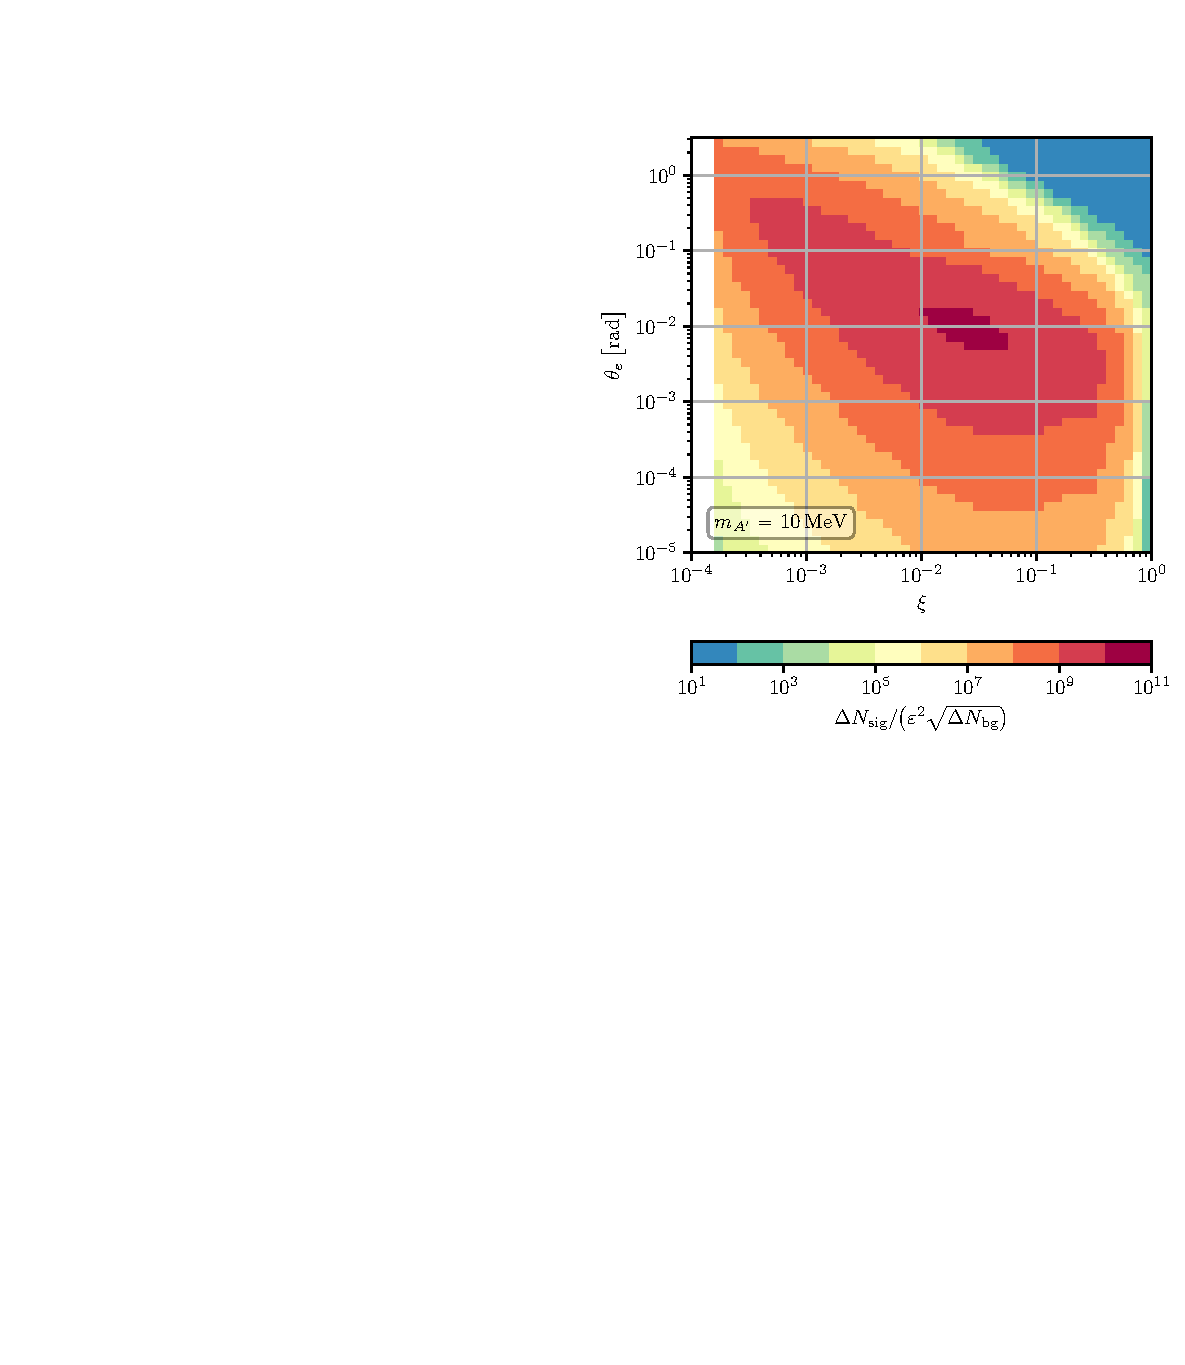
\includegraphics[width=0.95\linewidth]{plots/SB_Lohengrin.pdf}
\caption{Differential signal to background ratio as a function of electron kinematics for the production of a $10~{\rm MeV}$ Dark-photon at the hypothetical Lohengrin experiment.}
\label{fig:lohengrin}
\end{center}
\end{figure}


%
%\subsubsection{Cubic Higgs self interaction in Higgs plus jet at two loops}
%\begin{Namen}
%U. Haisch, M. Niggetiedt
%\end{Namen}
%
%{\color{red} ===========================\\ ==\; REMOVE? $\rightarrow$ IN ULI's REPORT\; ==\\ ===========================}
%
\printbibliography[heading=subbibliography]
\end{refsection}


% ----------------------------------------------------------------------
\clearpage
\onecolumn
% ----------------------------------------------------------------------
\end{document}
% ----------------------------------------------------------------------
